\documentclass[10pt, compress,spanish]{beamer}

\usetheme{cern}
% \usecolortheme{lily}



\usepackage[spanish, es-tabla]{babel}
\usepackage[utf8]{inputenc}
\usepackage{amsfonts}
\usepackage{amssymb}
\usepackage{amsmath}
\usepackage{amsbsy}
\usepackage{time}
\usepackage{rotating}
\usepackage{epsfig}
\usepackage{pifont}
\usepackage{verbatim}
\usepackage{pstricks}
\usepackage{multirow}
\usepackage{units}    
\usepackage{threeparttable}
\usepackage{mathrsfs}    
\usepackage{fancyhdr}
\usepackage{cite}
\usepackage{array}
\usepackage{graphicx}
\usepackage{graphics}
\usepackage{gensymb}
\usepackage{subcaption}
\usepackage{caption}
\usepackage{changepage}
\usepackage{minibox}

\usepackage{setspace}

\usepackage{tikz} 
\usetikzlibrary{shapes,arrows,positioning,automata,backgrounds,calc,er,patterns}
\usepackage{tikz-feynman}
\tikzfeynmanset{compat=1.0.0}

\usepackage{mathtools}
\DeclarePairedDelimiter\bra{\langle}{\rvert}
\DeclarePairedDelimiter\ket{\lvert}{\rangle}
\DeclarePairedDelimiterX\braket[2]{\langle}{\rangle}{#1 \delimsize\vert #2}

\newcolumntype{P}[1]{>{\centering\arraybackslash}p{#1}}




\title[Tesis de Licenciatura]
{Estudios de fondos de electrones reconstruidos como fotones en búsquedas de Supersimetría con el detector ATLAS}
\author{Orellana, Gonzalo \\
		Wahlberg, Hern\'an 
		}
\date{ }

\institute{UNLP}

\begin{document}

%%%%%%%%%%%%%%%%%%%%%%%%%%%%%%%%%%%%%%%%%%%%%%%%%%%%%%%%%%%%%%%%%%%%%%%%%%%%%%%%%%%%%%%%%%%%%%%%%%%%%%%%%%%%%%

% \frame{\titlepage}

\begin{frame}

\addtocounter{framenumber}{-1}

\hrulefill
\vspace{0.5cm}

  \begin{beamercolorbox}[leftskip=\titlelf]{title}
    \centering\usebeamerfont{title}\inserttitle
  \end{beamercolorbox}


\hrulefill

% \vspace{0.5cm}

\centering\footnotesize Facultad de Ciencias Exactas, UNLP

Tesis de Licenciatura en Física


\vspace{1cm}
\centering \normalsize Orellana, Gonzalo E.



\vspace{0.5cm}
\small Director\\
\normalsize Wahlberg, Hernán P.

\vspace{1cm}
\footnotesize Agradecimiento especial a Francisco Alonso \\

\end{frame}

%%%%%%%%%%%%%%%%%%%%%%%%%%%%%%%%%%%%%%%%%%%%%%%%%%%%%%%%%%%%%%%%%%%%%%%%%%%%%%%%%%%%%%%%%%%%%%%%%%%%%%%%%%%%%%


\begin{frame}{Tabla de contenidos}
\normalsize
\tableofcontents
\end{frame}

%%%%%%%%%%%%%%%%%%%%%%%%%%%%%%%%%%%%%%%%%%%%%%%%%%%%%%%%%%%%%%%%%%%%%%%%%%%%%%%%%%%%%%%%%%%%%%%%%%%%%%%%%%%%%%
\section{Marco Teórico}
\subsection{Modelo Estándar}
\begin{frame}[fragile]

\frametitle{Partículas del Modelo Estándar}

\normalsize

\renewcommand{\arraystretch}{1.3}
\begin{table} 
\centering\resizebox{\linewidth}{!}{
\begin{tabular}{ c  l | c  c  c | c c }

  \hline
  \hline

  &  & \multicolumn{3}{c |}{Partículas} & Espín & Carga eléctrica \\

  \hline
  \hline

  \multirow{5}{*}{\begin{sideways} Fermiones~ \end{sideways}} & \multirow{3}{*}{Quarks} & $(u,d)_{L}$ & $(c,s)_{L}$ & $(t,b)_{L}$ & $(\frac{1}{2},\frac{1}{2})$ & $(\frac{2}{3},-\frac{1}{3})$ \\

   &           & $u_{R}$ & $c_{R}$ & $t_{R}$ & $\frac{1}{2}$ & $\frac{2}{3}$ \\

  &            & $d_{R}$ & $s_{R}$ & $b_{R}$ & $\frac{1}{2}$ & $-\frac{1}{3}$ \\

  \cline{2-7}

  & \multirow{2}{*}{Leptones}   & $(\nu_{e},e^{-})_{L}$ & $(\nu_{\mu},\mu^{-})_{L}$ & $(\nu_{\tau},\tau^{-})_{L}$ & $(\frac{1}{2},\frac{1}{2})$ & $(0,-1)$ \\

  &              & $e_{R}^{-}$ & $\mu_{R}^{-}$ & $\tau_{R}^{-}$ & $\frac{1}{2}$ & $-1$ \\

  \hline
  \hline

  \multicolumn{2}{l |}{\multirow{3}{*}{Bosones de Gauge} }  & \multicolumn{3}{c |}{$g$} & $1$ & $0$ \\

   &                 & \multicolumn{3}{c |}{$W^{\pm}$, $Z$} & $1$ & $\pm1, 0$ \\

   &                 & \multicolumn{3}{c |}{$\gamma$} & $1$ & $ 0$ \\

  \hline

  \multicolumn{2}{l |}{Bosones escalares} & \multicolumn{3}{c |}{$H$} & 0 & 0 \\

  \hline
  \hline

\end{tabular}}
\end{table}
\renewcommand{\arraystretch}{1}

\begin{block}{Interacciones asociadas a bosones de gauge:}

Electromagnética $\leftrightarrow$ Fotón

Débil $\leftrightarrow$ $W^{\pm}$, $Z$

Fuerte $\leftrightarrow$ Gluones

Gravitatoria $\leftrightarrow$ Gravitón (?)

\end{block}


\end{frame}



%%%%%%%%%%%%%%%%%%%%%%%%%%%%%%%%%%%%%%%%%%%%%%%%%%%%%%%%%%%%%%%%%%%%%%%%%%%%%%%%%%%%%%%%%%%%%%%%%%%%%%%%%%%%%%


% \subsection{Problemáticas del Modelo Estándar}
\begin{frame}[fragile]

\frametitle{Problemáticas del Modelo Estándar}

\normalsize

\begin{block}{Teóricos}
\begin{itemize}

  \item Problema de jerarquía ($M_{W}/M_{P} \simeq 10^{-17} \text{GeV}$)

  \item Problema de naturalidad

  \item Integración de la fuerza gravitatoria

  \item Gran cantidad de parámetros libres (19), por qué los fermiones izquierdos se agrupan en dobletes y los derechos en singletes, por qué hay tres cargas de color, cuántas generaciones hay, etc.

\end{itemize}
\end{block}

\begin{block}{Experimentales}
\begin{itemize}

  \item Materia oscura

  \item Neutrinos masivos

\end{itemize}
\end{block}

\end{frame}



%%%%%%%%%%%%%%%%%%%%%%%%%%%%%%%%%%%%%%%%%%%%%%%%%%%%%%%%%%%%%%%%%%%%%%%%%%%%%%%%%%%%%%%%%%%%%%%%%%%%%%%%%%%%%%

% \subsection{Divergencias cuadráticas en el modelo}

\begin{frame}[fragile]

\frametitle{Divergencias cuadráticas}

\small Correcciones cuánticas a un \textit{loop} al parámetro de masa del Higgs $m_{H}^{2}$ debido a la masa de un fermión de Dirac \textit{f} (izquierda) y debido a la masa de un campo escalar \textit{S} (derecha).

\normalsize

\begin{columns}

\begin{column}{0.5\textwidth}


\begin{figure}
  \centering
\resizebox{1\textwidth}{!}{
  \begin{tikzpicture}
  \begin{feynman}
  \vertex (a) {\(H\)};
  \vertex [right=2cm of a] (b);
  \vertex [above right=of b] (e);
  \vertex [below right=of b] (f);
  \vertex [above right=of f] (c);
  \vertex [right=2cm of c] (d);
  \diagram* {
  (a)-- [scalar] (b),
  (b)-- [fermion, quarter left, edge label=\(f\)] (e),
  (e)-- [quarter left] (c),
  (c)-- [quarter left, fermion] (f),
  (f)-- [quarter left] (b),
  (c)-- [scalar] (d),
  };
  \end{feynman}
  \end{tikzpicture}}
\end{figure}

\begin{figure}
  \centering
\resizebox{1\textwidth}{!}{
  \begin{tikzpicture}[scale=0.2\textwidth]
  \begin{feynman}
  \vertex (a) {\(H\)};
  \vertex [right=3cm of a] (b);
  \vertex [above left=of b] (d);
  \vertex [above right=of b] (f);
  \vertex [above right=of d] (e);
  \vertex [right=3cm of b] (c);
  \diagram* {
  (a)-- [scalar] (b),
  (b)-- [scalar, quarter left] (d),
  (d)-- [quarter left, scalar, edge label=\(S\)] (e),
  (e)-- [quarter left, scalar] (f),
  (f)-- [quarter left, scalar] (b),
  (b)-- [scalar] (c),
  };
  \end{feynman}
  \end{tikzpicture}}
  \end{figure}

\begin{equation*}
\Delta m_{H}^{2}=-\frac{|\lambda_{f}|^{2}}{8\pi^{2}}\Lambda_{UV}^{2}+...
\end{equation*}

\end{column}


\begin{column}{0.5\textwidth} 

\vspace{-0.5cm}

\begin{equation*}
\Delta m_{H}^{2}=-\frac{|\lambda_{f}|^{2}}{8\pi^{2}}\Lambda_{UV}^{2}+...
\end{equation*}

Si $\Lambda_{UV} \sim M_{P} \longrightarrow$ la correción es 30 órdenes de magnitud más grande de lo esperado
  
\vspace{0.5cm}

\begin{equation*}
\Delta m_{H}^{2}=\frac{\lambda_{S}}{16\pi^{2}}\Lambda_{UV}^{2} + ...
\end{equation*}

\vspace{0.2cm}

  \begin{beamercolorbox}[leftskip=\titlelf]{title}
    \centering\usebeamerfont{title}\normalsize Supersimetría como extensión del SM
  \end{beamercolorbox}

\end{column}
\end{columns}


\end{frame}



%%%%%%%%%%%%%%%%%%%%%%%%%%%%%%%%%%%%%%%%%%%%%%%%%%%%%%%%%%%%%%%%%%%%%%%%%%%%%%%%%%%%%%%%%%%%%%%%%%%%%%%%%%%%%%

\subsection{SUSY}

\begin{frame}[fragile]
\frametitle{Supersimetría (SUSY)}

\normalsize

% Existencia de fermiones (bosones) no predichos por el SM, relacionados con los bosones (fermiones) del SM mediante una supersimetría

% \vspace{1cm}


\begin{columns}

\begin{column}{0.5\textwidth} 
Existencia de fermiones (bosones) no predichos por el SM, relacionados con los bosones (fermiones) del SM mediante una supersimetría

\end{column}

\begin{column}{0.5\textwidth} 
\begin{figure}
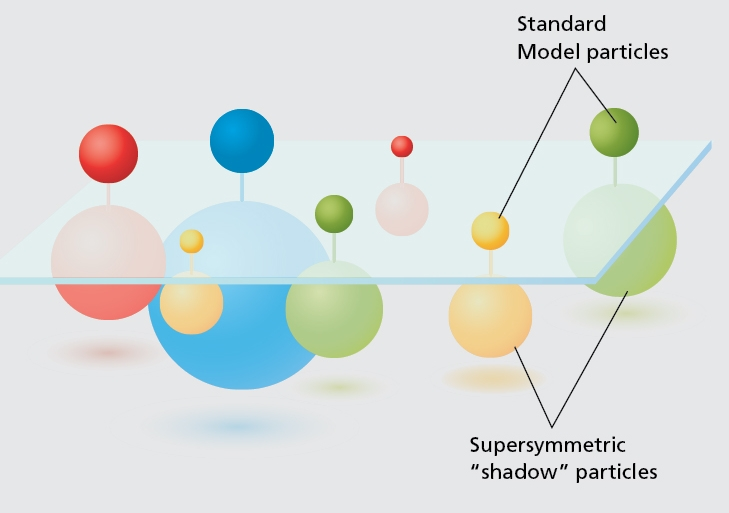
\includegraphics[width=0.9\textwidth]{supersymmetry2.jpg}
\end{figure}
\end{column}

\end{columns}

\begin{block}{Operador que genera la transformación:}
\begin{equation*}
\centering
Q \ket{\text{\,bosón\,}} = \ket{\text{\,fermión\,}}
\qquad\qquad\qquad
Q \ket{\text{\,fermión\,}} = \ket{\text{\,bosón\,}}
\end{equation*}
\end{block}

\vspace{0.3cm}

\begin{itemize}

  \item Supermultiplete con ambos estados bosón y fermión

  \item Misma carga eléctrica, carga de color e isospín.

  \item Misma masa...

\end{itemize}




\end{frame}


%%%%%%%%%%%%%%%%%%%%%%%%%%%%%%%%%%%%%%%%%%%%%%%%%%%%%%%%%%%%%%%%%%%%%%%%%%%%%%%%%%%%%%%%%%%%%%%%%%%%%%%%%%%%%%

% \subsection{MSSM}

\begin{frame}[fragile]

\frametitle{Modelo Estándar Supersimétrico Mínimo (MSSM)}

\normalsize

\renewcommand{\arraystretch}{1.3}
\begin{table} 
\centering\resizebox{\textwidth}{!}{
\begin{tabular}{ P{4cm} | P{4cm} | P{4cm} }

  \hline
  \hline

  Supermultiplete & Bosón & Fermión \\

  \hline
  \hline

  gluón, gluino & $g$ & $\widetilde{g}$ \\

  \hline

  W, wino & $W^{\pm}$, $W^{0}$ & $\widetilde{W}^{\pm}$, $\widetilde{W}^{0}$ \\
  B, bino & B & $\widetilde{B}$ \\

  \hline

  \multirow{2}{*}{sleptón, leptón $^{*}$}   & $(\widetilde{\nu},\widetilde{e})_{L}$ & $(\nu,e)_{L}$ \\

                    & $\widetilde{e}_{R}$ & $e_{R}$ \\

  \hline

  \multirow{3}{*}{squark, quark $^{*}$}   & $(\widetilde{u}_{L},\widetilde{d}_{L})$ & $(u_{L},d_{L})$ \\

                    & $\widetilde{u}_{R}$ & $u_{R}$ \\

                    & $\widetilde{d}_{R}$ & $d_{R}$ \\

  \hline

  \multirow{2}{*}{Higgs, higgsinos} & $(H^{0}_{d},H^{-}_{d})$ & $(\widetilde{H}^{0}_{d},\widetilde{H}^{-}_{d})$ \\

                    & $(H^{+}_{u},H^{0}_{u})$ & $(\widetilde{H}^{+}_{u},\widetilde{H}^{0}_{u})$ \\

  \hline
  \hline
\end{tabular}}
\end{table}

\renewcommand{\arraystretch}{1}

% \vspace{0.8cm}
\footnotesize{$^{*}$ Junto con las otras dos generaciones}

\begin{block}{\normalsize Los supercompañeros tienen la misma masa y por ende deberían haber sido observados...}
\end{block}

\end{frame}



%%%%%%%%%%%%%%%%%%%%%%%%%%%%%%%%%%%%%%%%%%%%%%%%%%%%%%%%%%%%%%%%%%%%%%%%%%%%%%%%%%%%%%%%%%%%%%%%%%%%%%%%%%%%%%

% \subsection{Estados de masa}

\begin{frame}[fragile]

\frametitle{Estados de masa}

  \begin{beamercolorbox}[leftskip=\titlelf]{title}
    \centering\usebeamerfont{title}\normalsize SUSY $\longrightarrow$ simetría rota
  \end{beamercolorbox}


\begin{equation*}
\mathcal{L}=\mathcal{L}_{\text{SUSY}}+\mathcal{L}_{\text{soft}}
\end{equation*}

\normalsize

\vspace{0.5cm}

Ejemplo de modelo de ruptura: “Generalised Model of Gauge-Mediated Supersymmetry Breaking” (GGMSB) 
{\footnotesize ($\tilde{G}$=LSP, $\chi_{1}^{0}$=NLSP)}

\vspace{0.5cm}

\begin{columns}

\begin{column}{0.5\textwidth}
\begin{itemize}

  \item Sector de Higgs: $H^{\pm}$,  $A^{0}$,  $H^{0}$ y $h^{0}$

  \item Neutralinos y charginos: $\widetilde{\chi}^{0}_{1}$, $\widetilde{\chi}^{0}_{2}$, $\widetilde{\chi}^{0}_{3}$, $\widetilde{\chi}^{0}_{4}$ y $\widetilde{\chi}^{\pm}_{1}$, $\widetilde{\chi}^{\pm}_{2}$

  \item Gluino

  \item Squarks y sleptones


\end{itemize}
\end{column}

\begin{column}{0.5\textwidth}



\begin{figure}
\centering
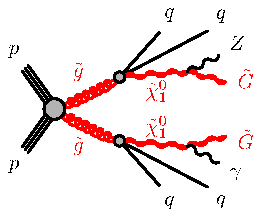
\includegraphics[width=0.7\textwidth]{gogo-qqqqphZGG-GMSB.pdf}
\end{figure}


\end{column}
\end{columns}

\end{frame}



%%%%%%%%%%%%%%%%%%%%%%%%%%%%%%%%%%%%%%%%%%%%%%%%%%%%%%%%%%%%%%%%%%%%%%%%%%%%%%%%%%%%%%%%%%%%%%%%%%%%%%%%%%%%%%


\section{Experimento}

\subsection{LHC}

\begin{frame}[fragile]
\frametitle{Gran Colisionador de Hadrones (LHC)}

\normalsize

\begin{figure}
\centering
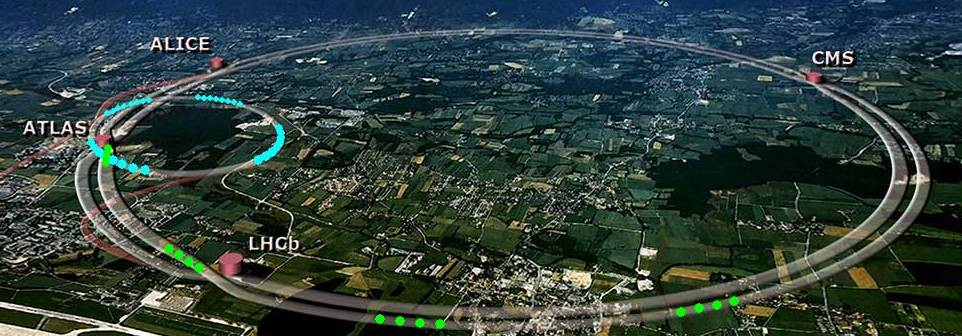
\includegraphics[width=0.9\textwidth]{lhc-sim.jpg}
\end{figure}

\begin{beamercolorbox}[leftskip=\titlelf]{title}
\centering\usebeamerfont{title}\normalsize Acelera protones (iones) en un anillo subterráneo de 27 km de longitud y los hace colisionar en 4 puntos distintos, donde se encuentran diferentes tipos de detectores
\end{beamercolorbox}


\vspace{1cm}
\centering

Run 2

$\sqrt{s}=13\:\text{TeV}$

$\mathcal{L} = 1.4\cdot 10^{34}$ cm$^{-2}$s$^{-1}$


\end{frame}



%%%%%%%%%%%%%%%%%%%%%%%%%%%%%%%%%%%%%%%%%%%%%%%%%%%%%%%%%%%%%%%%%%%%%%%%%%%%%%%%%%%%%%%%%%%%%%%%%%%%%%%%%%%%%%

\subsection{ATLAS}

\begin{frame}[fragile]
\frametitle{Detector ATLAS}

\normalsize


\begin{figure}
\centering
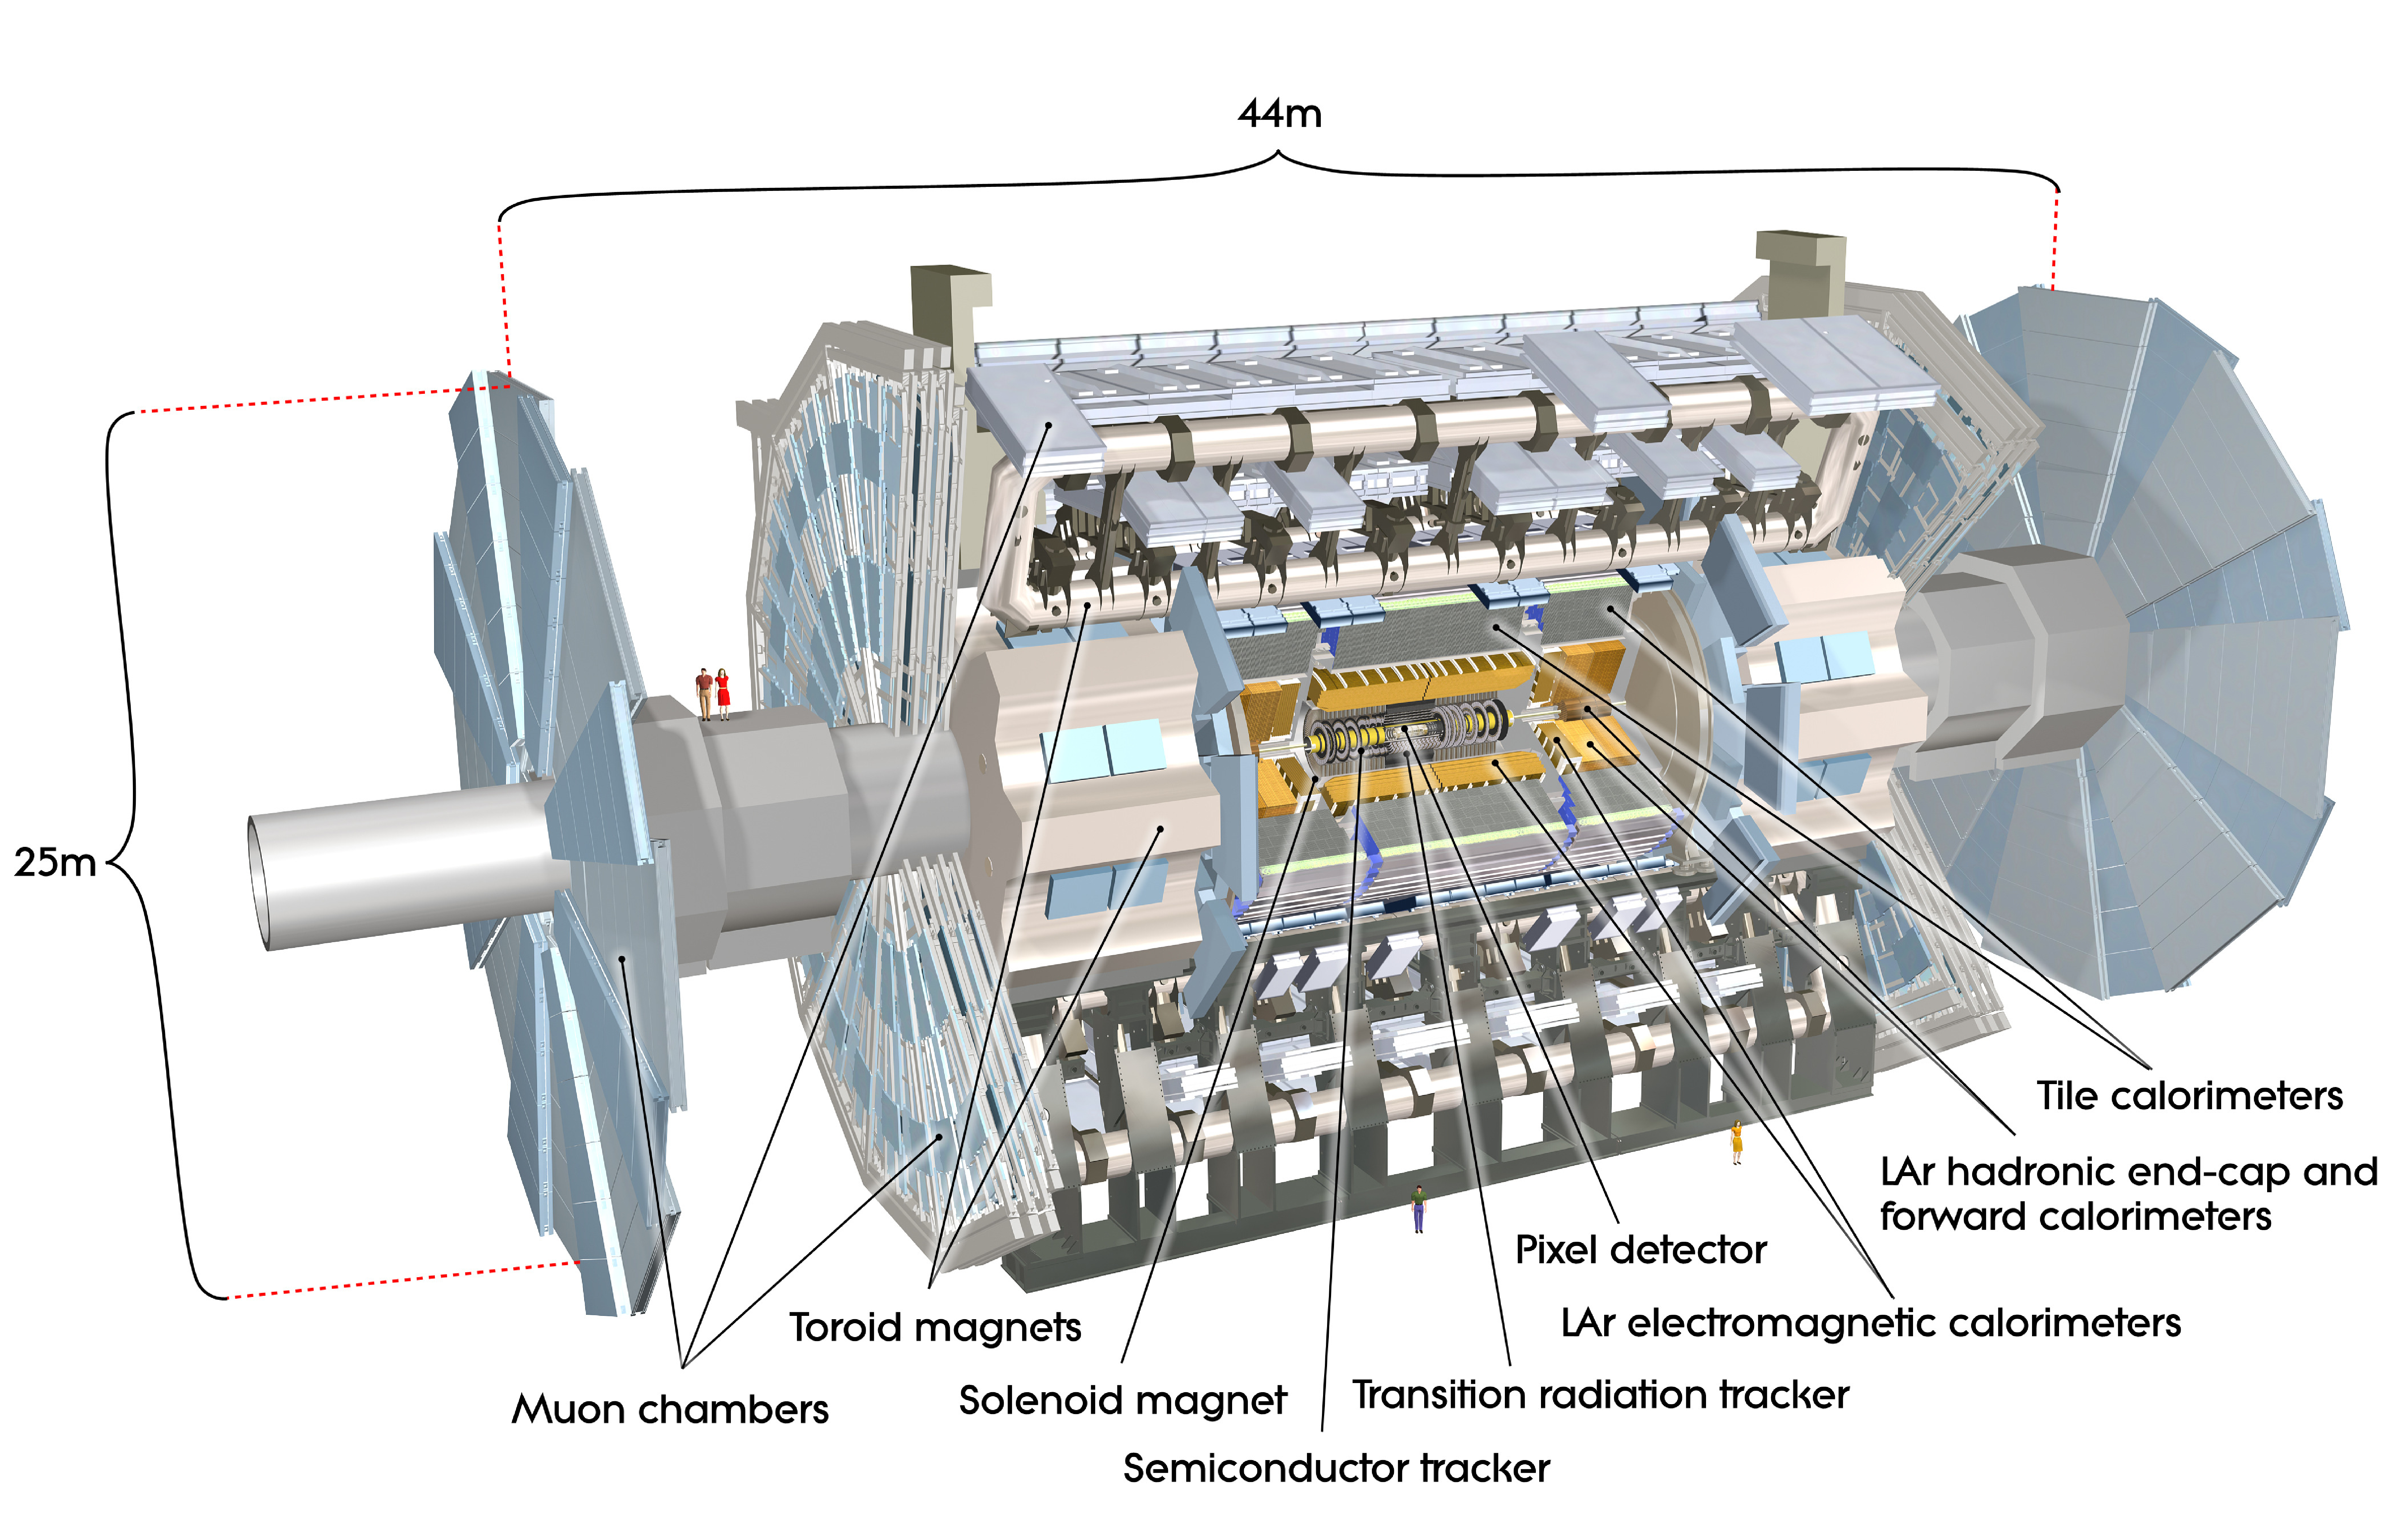
\includegraphics[width=0.8\textwidth]{ATLAS-eps-converted-to.pdf}
\label{ATLAS}
\end{figure}


Subdetectores:
\begin{itemize}

  \item Detector Interno: IBL, Píxel, SCT, TRT

  \item Calorímetros: ECAL, HCAL

  \item Espectrómetro de muones

\end{itemize}


\end{frame}



%%%%%%%%%%%%%%%%%%%%%%%%%%%%%%%%%%%%%%%%%%%%%%%%%%%%%%%%%%%%%%%%%%%%%%%%%%%%%%%%%%%%%%%%%%%%%%%%%%%%%%%%%%%%%%


% \subsubsection{ID}
\begin{frame}[fragile]
\frametitle{Detector interno}

\small

\begin{figure}
\centering
  \begin{subfigure}{0.45\textwidth}
    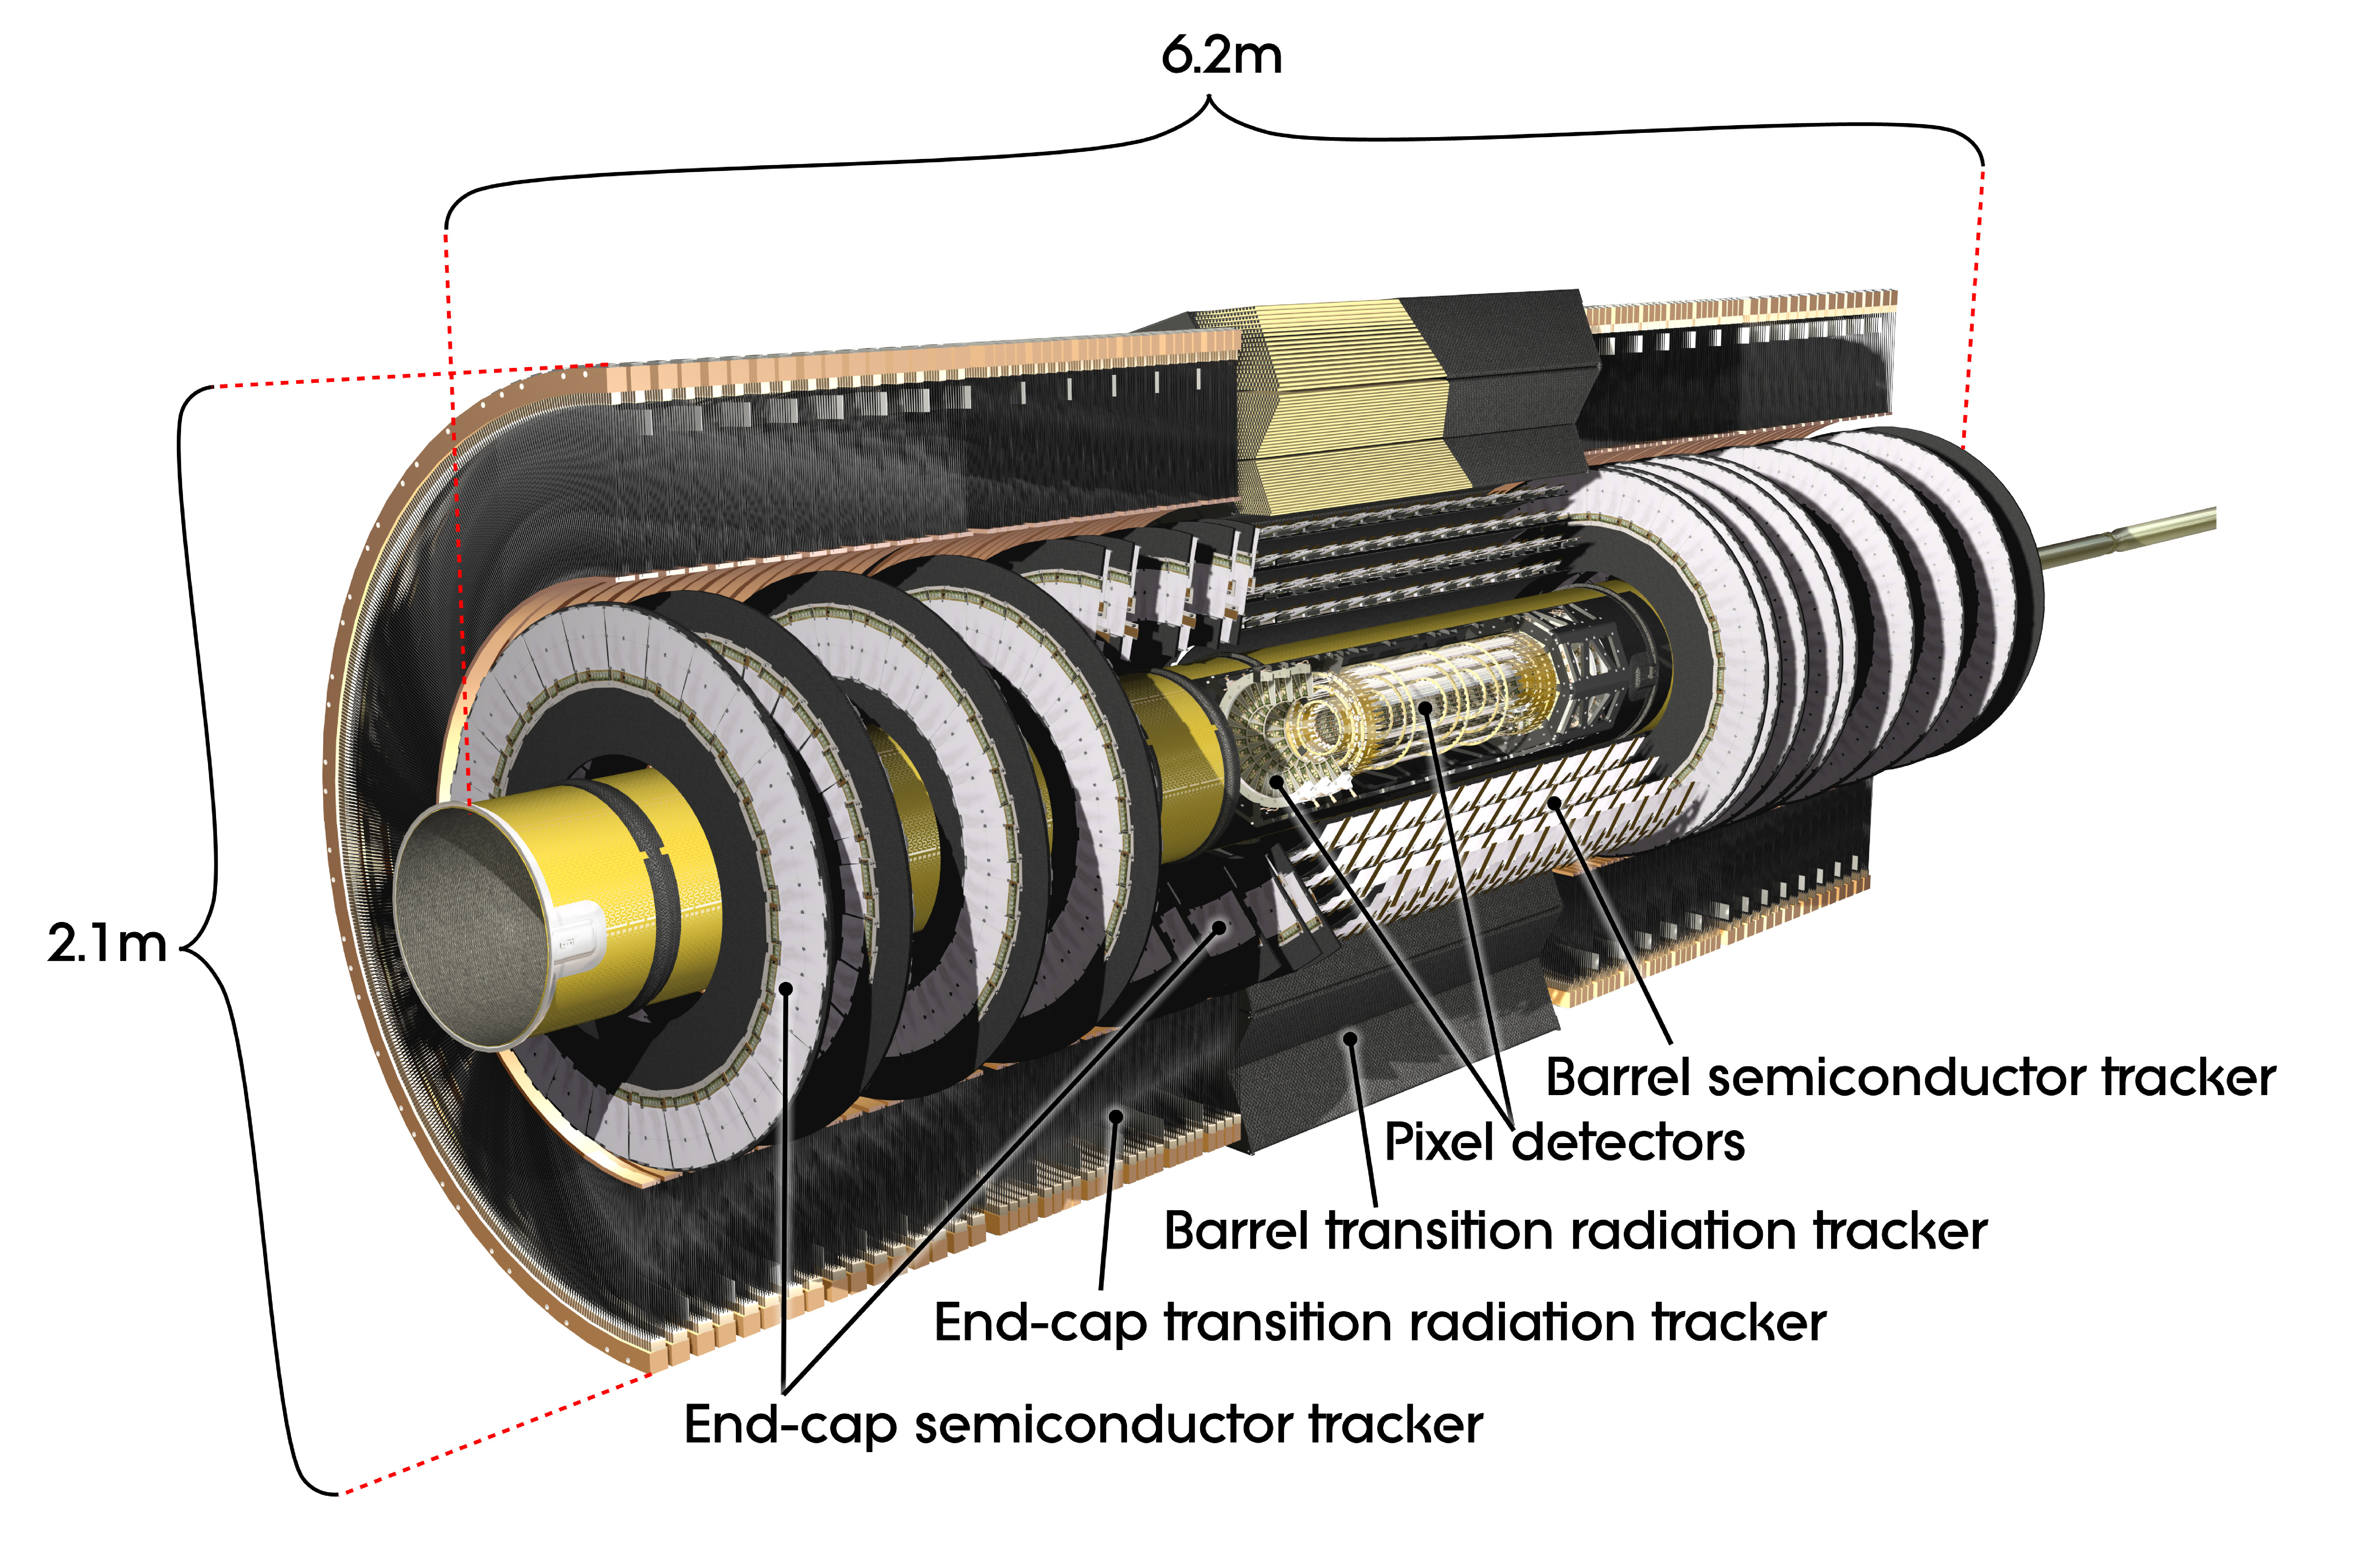
\includegraphics[scale=0.045]{ID-eps-converted-to.pdf} 
  \end{subfigure}
  \hfill
  \begin{subfigure}{0.45\textwidth}
    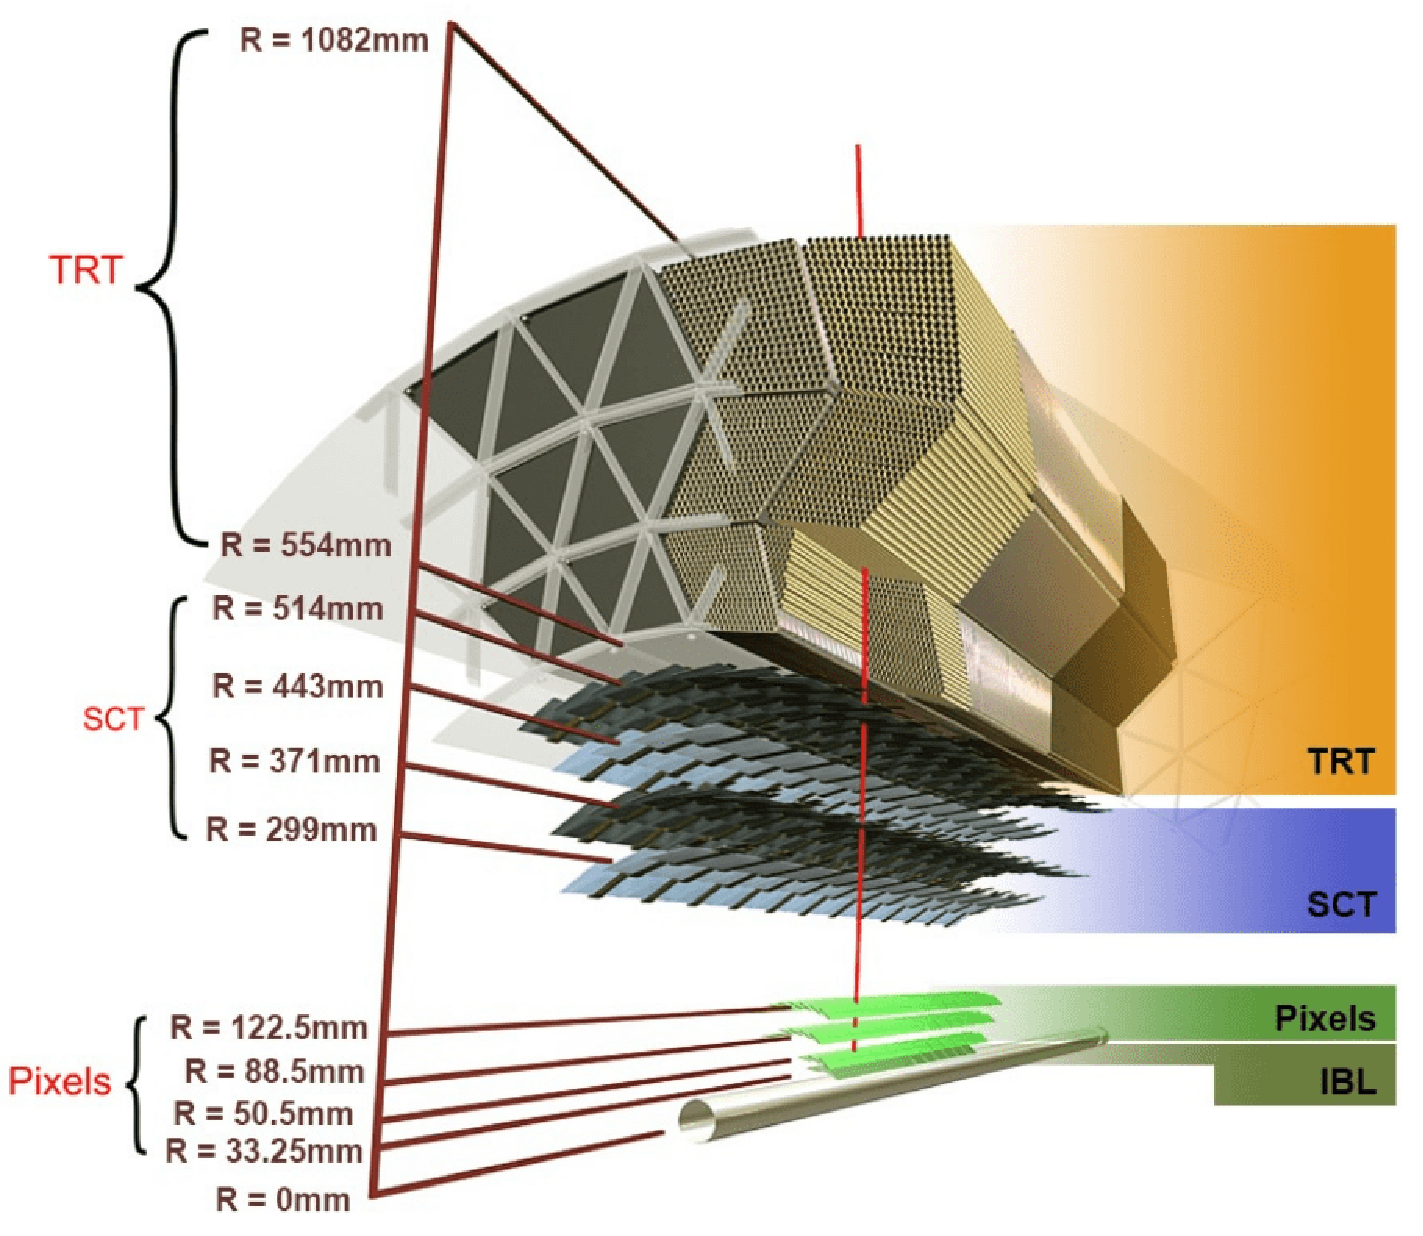
\includegraphics[scale=0.2]{ID_2.pdf}
  \end{subfigure}
\end{figure}



\begin{itemize}

  \item Insertable B-Layer: chips + sensores de silicio. Resolución de $8\:\mu$m ($R-\phi$) y $40\:\mu$m ($z$)

  \item Detector de Píxeles: sensores de silicio. Resolución de $10\:\mu$m ($R-\phi$) y $115\:\mu$m ($z$)

  \item Detector Semiconductor de Trazas (SCT): sensores de silicio en microbandas. Resolución de $17\:\mu$m ($R-\phi$) y $580\:\mu$m ($z$)

  \item Detector de Radiación de Transición (TRT): tubos con gas ionizable. Resolución de $0.17$ mm. Diferencia entre partículas pesadas y livianas.

\end{itemize}



\end{frame}



%%%%%%%%%%%%%%%%%%%%%%%%%%%%%%%%%%%%%%%%%%%%%%%%%%%%%%%%%%%%%%%%%%%%%%%%%%%%%%%%%%%%%%%%%%%%%%%%%%%%%%%%%%%%%%


% \subsubsection{CALO}
\begin{frame}[fragile]
\frametitle{Sistema de calorímetros}

\normalsize

\begin{figure}
\centering
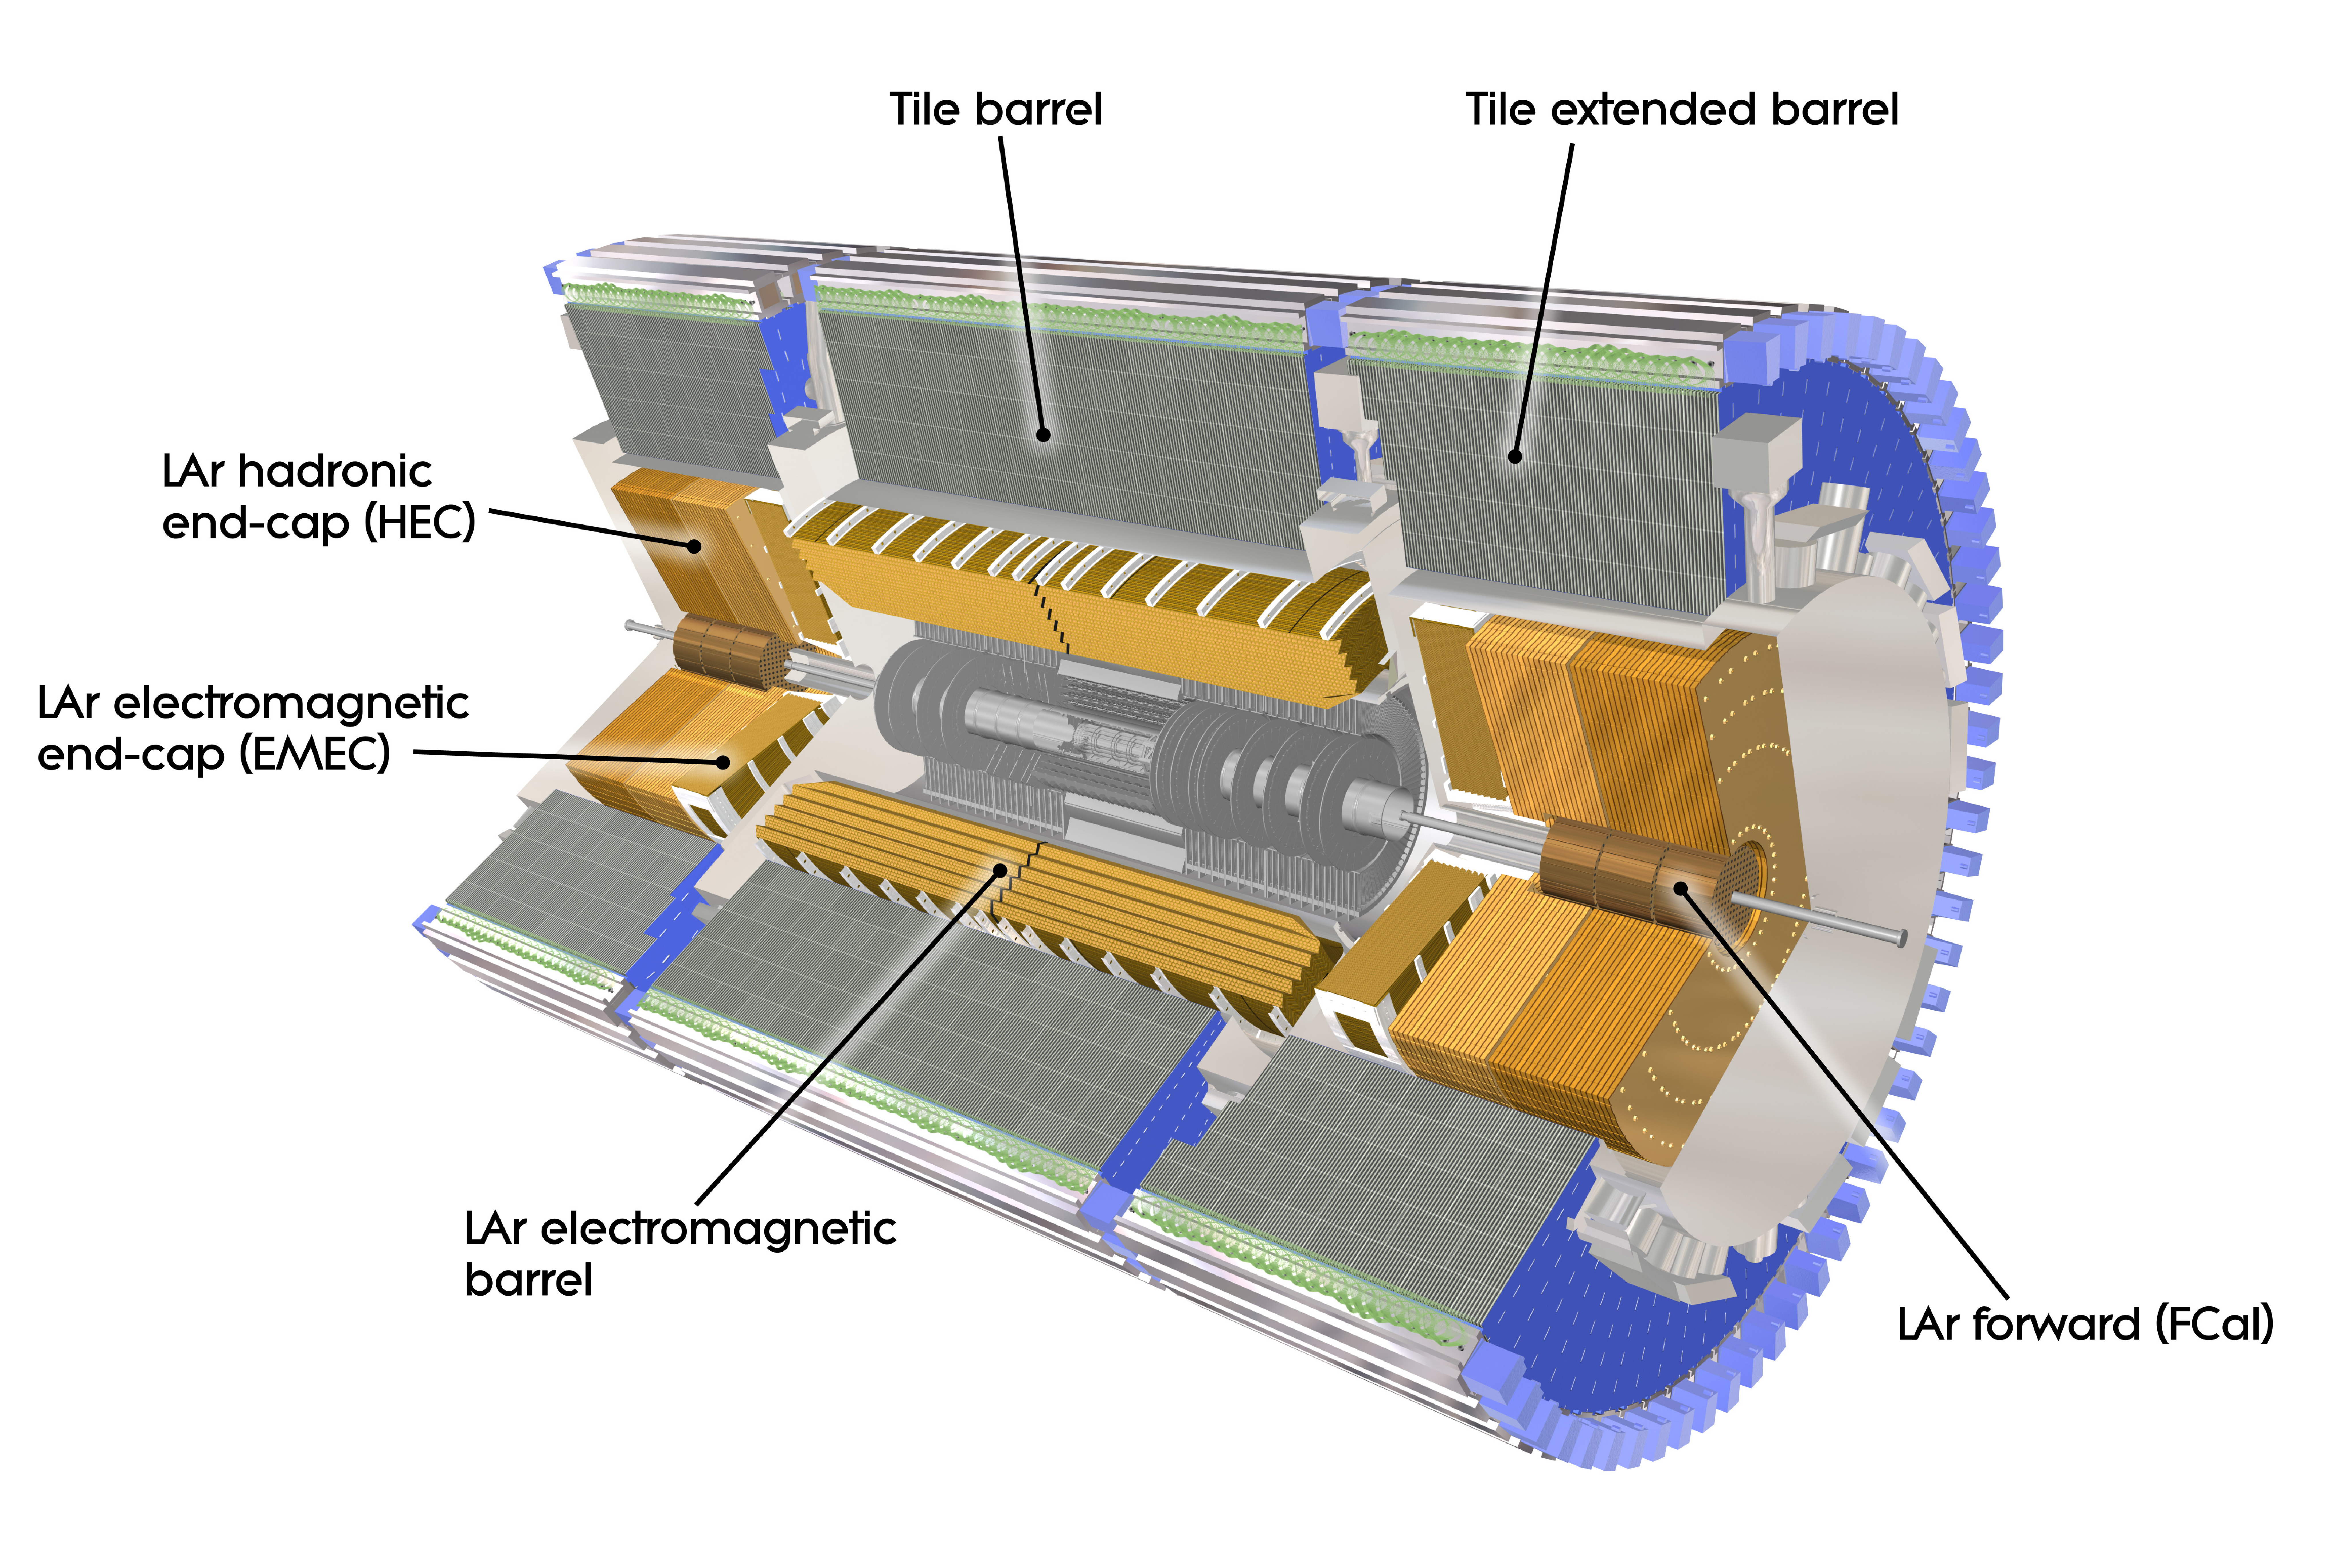
\includegraphics[width=0.73\textwidth]{Cal-eps-converted-to.pdf}
\end{figure}

\begin{beamercolorbox}[leftskip=\titlelf]{title}
\usebeamerfont{title}\normalsize Calorímetros de muestreo
\end{beamercolorbox}
Material absorbente + medio activo

\begin{itemize}

  \item Electromagnético (ECAL): plomo + LAr

  \item Hadrónico (HCAL): acero + tejas centelladoras plásticas / cobre + LAr

\end{itemize}




\end{frame}



%%%%%%%%%%%%%%%%%%%%%%%%%%%%%%%%%%%%%%%%%%%%%%%%%%%%%%%%%%%%%%%%%%%%%%%%%%%%%%%%%%%%%%%%%%%%%%%%%%%%%%%%%%%%%%

% \subsubsection{MS}
\begin{frame}[fragile]
\frametitle{Espectrómetro de muones}

\normalsize


\begin{figure}
\centering
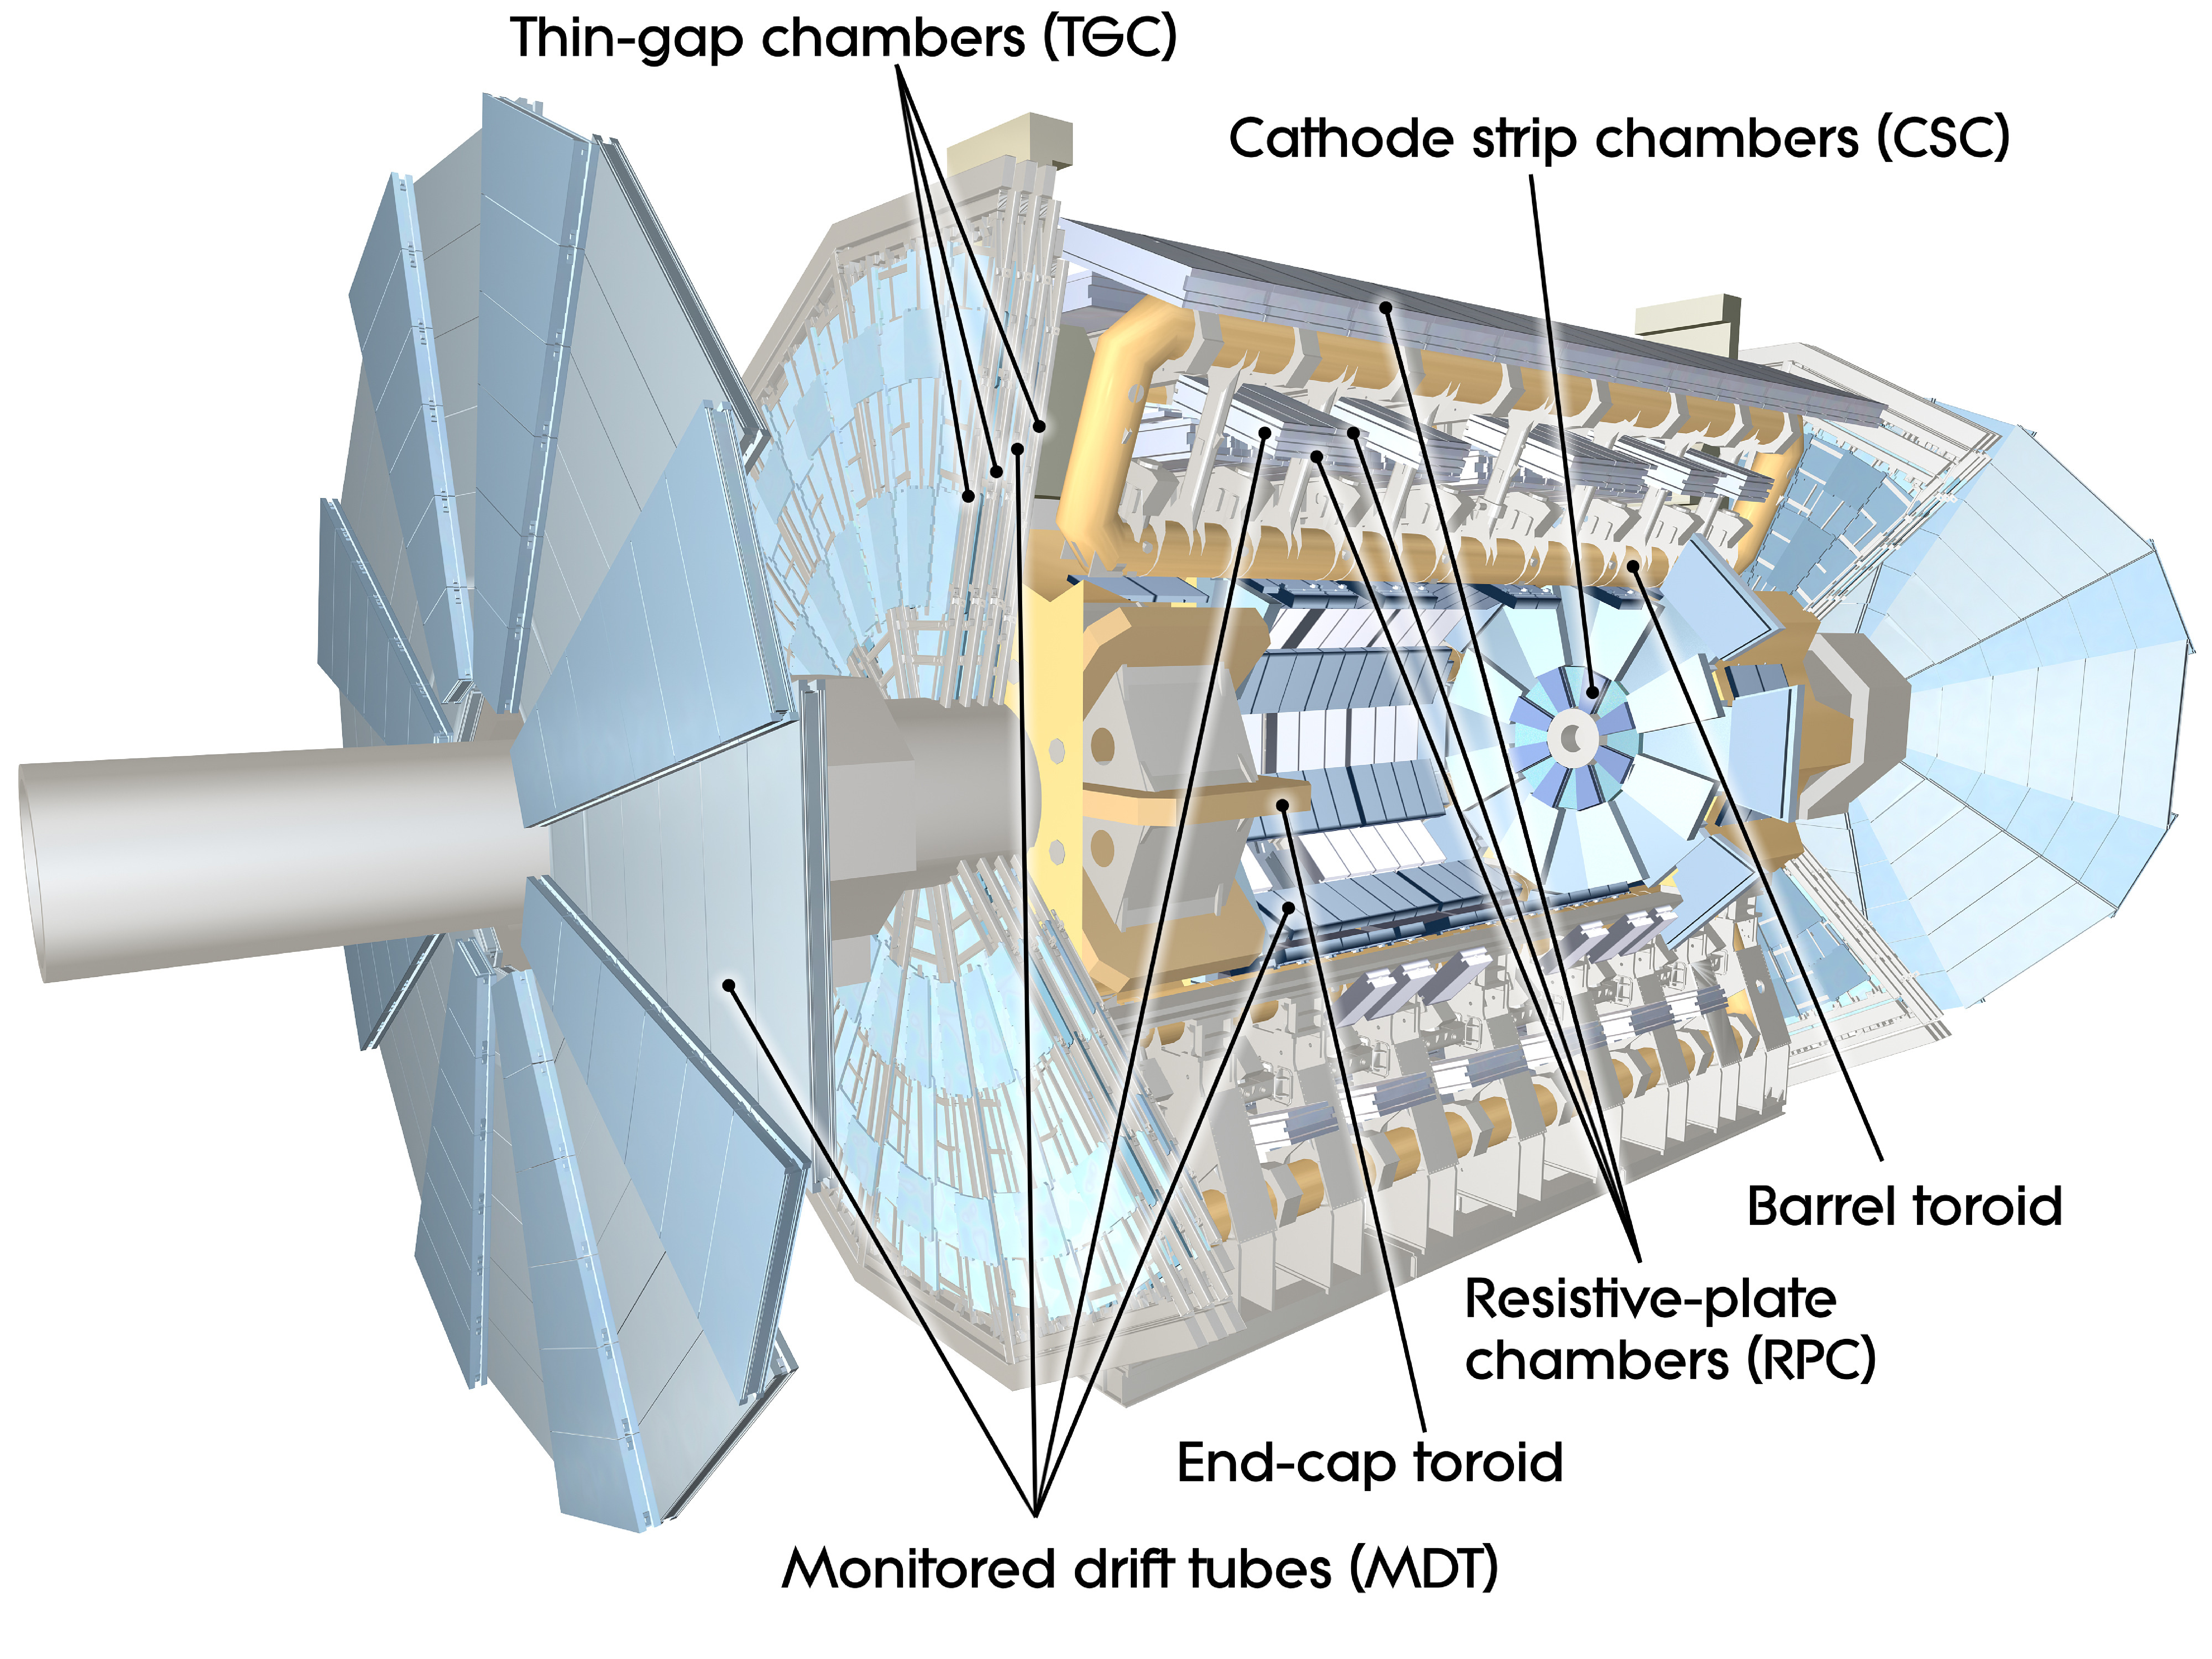
\includegraphics[width=0.55\textwidth]{muon-eps-converted-to.pdf}
\end{figure}

Cámaras de detección:
\begin{itemize}

  \item \textit{Monitored Drift Tubes} (MDTs)

  \item \textit{Cathode Strip Chambers} (CSCs)

  \item \textit{Resistive Plate Chamber} (RPCs)

  \item \textit{Thin Gap Chambers} (TGCs)

\end{itemize}


\end{frame}



%%%%%%%%%%%%%%%%%%%%%%%%%%%%%%%%%%%%%%%%%%%%%%%%%%%%%%%%%%%%%%%%%%%%%%%%%%%%%%%%%%%%%%%%%%%%%%%%%%%%%%%%%%%%%%


% \subsection{Trigger}
\begin{frame}[fragile]
\frametitle{Sistema de \textit{trigger}, adquisición y distribución de datos}

\small

\vspace{0.5cm}

\begin{beamercolorbox}[leftskip=\titlelf]{title}
\usebeamerfont{title}\normalsize Interacción $pp$
\end{beamercolorbox}
Frecuencia de cruce de haces 40 MHz y alrededor de 23 interacciones por cruce $\longrightarrow$ $\sim$1 GHz $\xrightarrow{reducir}$ $\sim 1.5$ kHz

% \vspace{0.3cm}


\begin{beamercolorbox}[leftskip=\titlelf]{title}
\usebeamerfont{title}\normalsize \textit{Trigger}
\end{beamercolorbox}
\begin{itemize}

  \item Level 1 (L1): basado en hardware (ECAL, HCAL y MS), $2.5 \:\mu$s, $\sim 100$ kHz

  \item \textit{High Level Trigger} (HLT): basado en algoritmos, $0.2$ s, $\sim 1.5$ kHz

\end{itemize}

% \vspace{0.3cm}

\begin{beamercolorbox}[leftskip=\titlelf]{title}
\usebeamerfont{title}\normalsize Distribución y procesamiento de datos adquiridos
\end{beamercolorbox}
\begin{itemize}

  \item tecnología GRID para distribución y procesamiento de datos

  \item HTL $\longrightarrow$ \textit{Raw Data Objects} (RDOs) $\longrightarrow$ ESD (\textit{Event Summary Data})/AOD (\textit{Analysis Object Data}) $\longrightarrow$ xAOD

  \item Entorno de ROOT

\end{itemize}

% \vspace{0.3cm}

\begin{beamercolorbox}[leftskip=\titlelf]{title}
\usebeamerfont{title}\normalsize Derivaciones
\end{beamercolorbox}
EGAM1: eventos optimizados para estudios del bosón $Z$, base de electrones y fotones con $p_{T} > 7 \:\text{GeV}$ y masa invariante de los distintos tipos de pares mayor a $50 \text{GeV}$...

\end{frame}



%%%%%%%%%%%%%%%%%%%%%%%%%%%%%%%%%%%%%%%%%%%%%%%%%%%%%%%%%%%%%%%%%%%%%%%%%%%%%%%%%%%%%%%%%%%%%%%%%%%%%%%%%%%%%%


% \subsection{RECO}
\begin{frame}[fragile]

\frametitle{Reconstrucción e identificación de electrones/fotones}

\normalsize

\begin{columns}
\begin{column}{0.4\textwidth}
\begin{block}{Reconstrucción:}
\begin{itemize}

\item Algoritmo de clusterización

\item Asociación \textit{cluster} con las trazas en el ID

\end{itemize}
\end{block}

\begin{block}{Identificación:}
\begin{itemize}

\item Fotones: \textit{loose} y \textit{tight}, cortes rectangulares

\item Electrones: \textit{loose}, \textit{medium} y \textit{tight}, método de \textit{likelihood}

\end{itemize}
\end{block}
\end{column}

\begin{column}{0.6\textwidth}
\begin{figure}
\centering
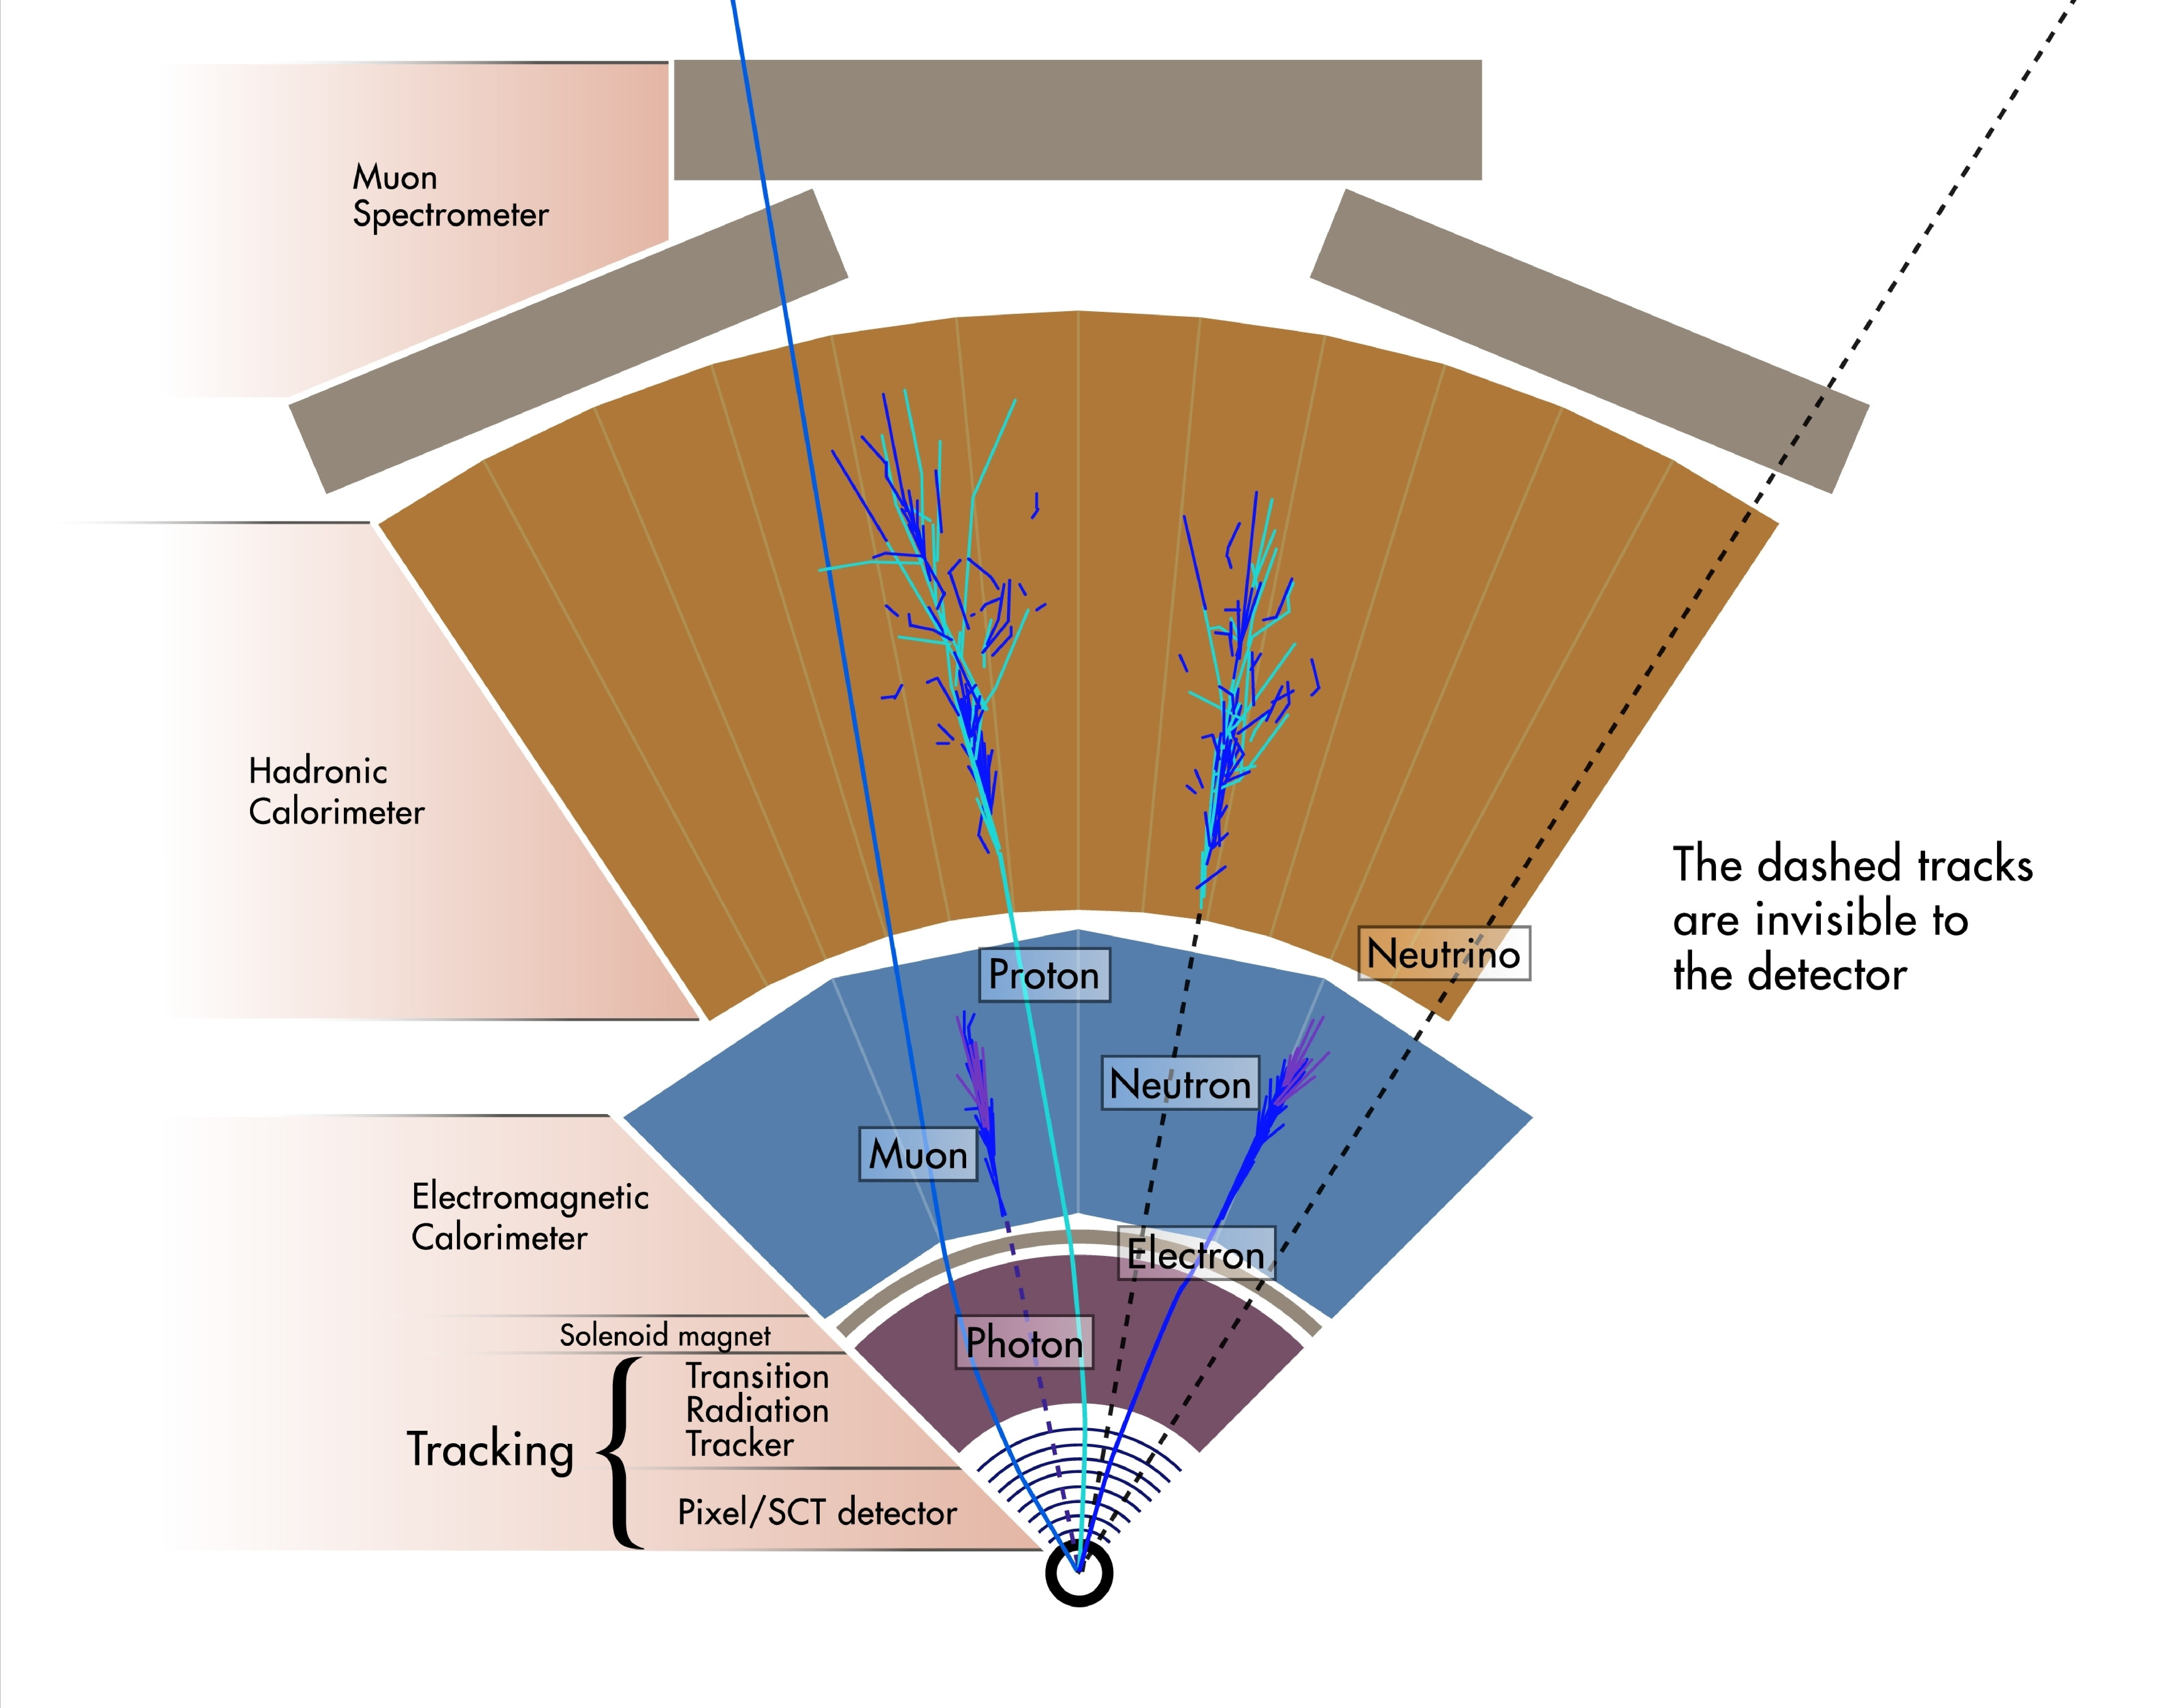
\includegraphics[width=1.15\textwidth]{cross_section_2-eps-converted-to.pdf}
\end{figure}
\end{column}

\end{columns}


\end{frame}


%%%%%%%%%%%%%%%%%%%%%%%%%%%%%%%%%%%%%%%%%%%%%%%%%%%%%%%%%%%%%%%%%%%%%%%%%%%%%%%%%%%%%%%%%%%%%%%%%%%%%%%%%%%%%%

\begin{frame}[fragile]

\frametitle{Variables de identificación}
\footnotesize
\vspace{-1.68cm}

\begin{columns}



\begin{column}{0.6\textwidth}

\begin{table} 
\centering
\centering\resizebox{1.\textwidth}{!}{
 \begin{tabular}{ r c | c c | c }

  \hline

  \multirow{2}{*}{Categoría}  & \multirow{2}{*}{Nombre} & \multicolumn{2}{ c |}{$\gamma$} & \multirow{2}{*}{$e$} \\

    & & L & T &   \\

  \hline

  Aceptancia &  - & $\times$ & $\checkmark$ & $\times$  \\

  Fuga hadrónica  & $R_{\text{had}_{1}}$ & $\checkmark$ & $\checkmark$ & $\checkmark$ \\

    & $R_{\text{had}}$ & $\checkmark$ & $\checkmark$ & $\checkmark$  \\

  ECAL (3$^{ra}$ capa) & $f_{3}$ & $\times$ & $\times$ & $\checkmark$  \\
  

  ECAL (2$^{da}$ capa) &  $w_{\eta_{2}}$ & $\checkmark$ & $\checkmark$ & $\checkmark$ \\

    & $R_{\eta}$ & $\checkmark$ & $\checkmark$ & $\checkmark$ \\

    &  $R_{\phi}$ & $\times$ & $\checkmark$ & $\checkmark$ \\

  ECAL (1$^{ra}$ capa) &  $w_{s,3}$ & $\times$ & $\checkmark$ & $\times$ \\

    &  $w_{s,\text{tot}}$ & $\times$ & $\checkmark$ & $\checkmark$ \\

    & $F_{\text{side}}$ & $\times$ & $\checkmark$ & $\times$ \\

    & $\Delta E$ & $\times$ & $\checkmark$ & $\times$ \\

    &  $\times$ & $\checkmark$ & $\checkmark$  \\

    &  $f_{1}$ & $\times$ & $\times$ & $\checkmark$  \\

  ID &  $d_{0}$ & $\times$ & $\times$ & $\checkmark$ \\

    &  $\Delta p/p$ & $\times$ & $\times$ & $\checkmark$  \\

  TRT &  eProbabilityHT & $\times$ & $\times$ & $\checkmark$  \\

  ECAL+ID &  $\Delta\eta_{1}$ & $\times$ & $\times$ & $\checkmark$ \\

  \hline

\end{tabular}}
\end{table}

\end{column}


\begin{column}{0.3\textwidth}

\begin{figure}
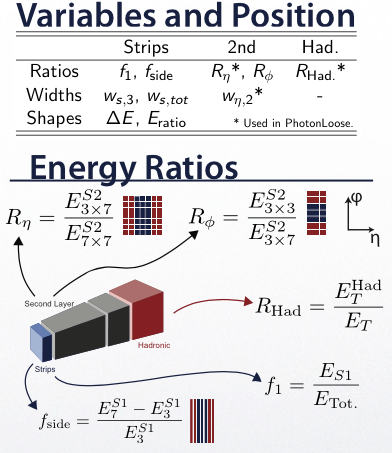
\includegraphics[scale=0.28]{EM_Showers1.png}
\end{figure}
\vspace{-1.2cm}
\begin{figure}
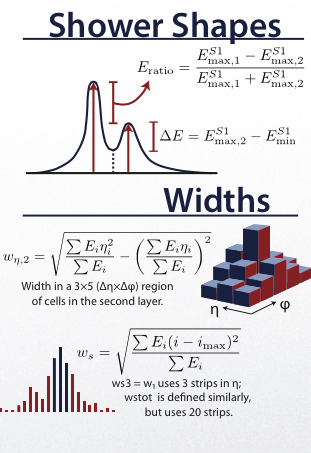
\includegraphics[scale=0.3]{EM_Showers2.png}
\end{figure}
\end{column}



\end{columns}





\end{frame}



%%%%%%%%%%%%%%%%%%%%%%%%%%%%%%%%%%%%%%%%%%%%%%%%%%%%%%%%%%%%%%%%%%%%%%%%%%%%%%%%%%%%%%%%%%%%%%%%%%%%%%%%%%%%%%

\begin{frame}[fragile]

\frametitle{Aislamiento}

\normalsize

\begin{beamercolorbox}[leftskip=\titlelf]{title}
\usebeamerfont{title}\normalsize Diferenciar electrones y fotones directos, de los no directos y de los mal reconstruidos
\end{beamercolorbox}

Cono de radio $R=\sqrt{\Delta\eta^{2}+\Delta\phi^{2}}$, centrado en el baricentro del cluster:

\begin{itemize}

\item Aislamiento de trazas

\item Aislamiento calorimétrico

\end{itemize}


\begin{columns}

\begin{column}{0.5\textwidth}
\begin{figure}
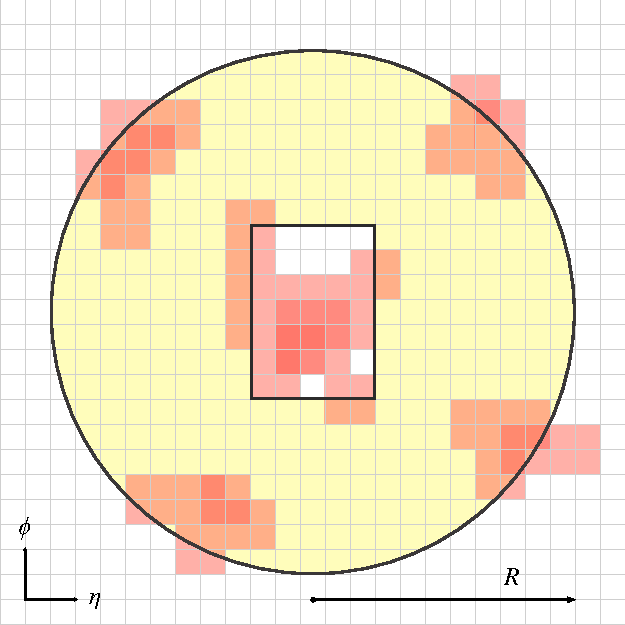
\includegraphics[scale=0.3]{iso.pdf}
\end{figure}
\end{column}


\begin{column}{0.5\textwidth}
\begin{figure}
\centering
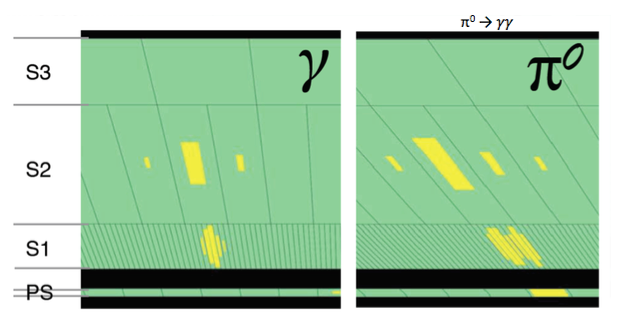
\includegraphics[width=1.15\textwidth]{Gamma_pi.png}
\end{figure}
\end{column}

\end{columns}

\begin{beamercolorbox}[leftskip=\titlelf]{title}
\usebeamerfont{title}\normalsize Clasificación de electrones y fotones
\end{beamercolorbox}
\begin{itemize}

\item Fotones: aislados, $E_{T}^{\text{iso}}<2.45 \text{GeV} + 0.022 \times p_{T}$

\item Electrones: \textit{Gradient Loose}

\end{itemize}




\end{frame}



%%%%%%%%%%%%%%%%%%%%%%%%%%%%%%%%%%%%%%%%%%%%%%%%%%%%%%%%%%%%%%%%%%%%%%%%%%%%%%%%%%%%%%%%%%%%%%%%%%%%%%%%%%%%%%

\begin{frame}[fragile]

\frametitle{Variables globales de selección de eventos}

\scriptsize


\begin{equation*}
p_{T}^{\text{miss}}=\left(p_{T}^{\text{miss}}\right)^{e} + \left(p_{T}^{\text{miss}}\right)^{\gamma} + \left(p_{T}^{\text{miss}}\right)^{\text{jet}} +\left(p_{T}^{\text{miss}}\right)^{\mu} + \left(p_{T}^{\text{miss}}\right)^{\text{soft}}
\end{equation*}

\begin{equation*}
E_{T}^{\text{miss}}=|p_{T}^{\text{miss}}|
\end{equation*}


\begin{equation*}
H_{T}=|p_{T}^{\gamma}|+\sum_{\text{jets}}|p_{T}^{\text{jet}}|
\end{equation*}


\centering 
$m_{\text{eff}}$: suma escalar de $H_{T}$ y $E_{T}^{\text{miss}}$


% \begin{equation*}
% R_{T}^{4}=\frac{\sum_{i}^{4}p_{T}^{i}}{\sum_{j}p_{T}^{j}}
% \end{equation*}

\hrulefill

\begin{figure}
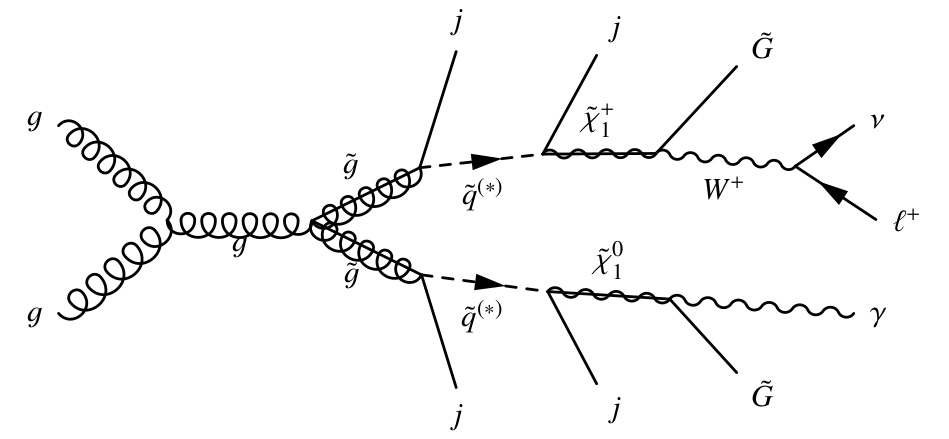
\includegraphics[width=0.7\textwidth]{feyn.png}
\end{figure}

\end{frame}



%%%%%%%%%%%%%%%%%%%%%%%%%%%%%%%%%%%%%%%%%%%%%%%%%%%%%%%%%%%%%%%%%%%%%%%%%%%%%%%%%%%%%%%%%%%%%%%%%%%%%%%%%%%%%%


\section{Estrategia general del análisis}

\begin{frame}[fragile]
\frametitle{Estrategia general del análisis de búsqueda de SUSY}

\normalsize

\begin{itemize}

\item Conteo del número de eventos observado en exceso sobre el SM en una cierta región del espacio de observables rica en eventos de la señal considerada.

\item Búsqueda de Supersimetría en eventos con al menos un fotón aislado muy energético, jets y gran cantidad de energía faltante en estado final.

\end{itemize}

\begin{table}
\centering
    \begin{tabular}{c|c|c} \hline
      & $E_{T}^{\text{miss}}$ real & $E_{T}^{\text{miss}}$ instrumental \\
      \hline
      Fotones reales &
      \begin{tabular}[c]{@{}c@{}}
        $Z(\to\nu\nu)\gamma$, $Z\gamma\gamma$, $W\gamma$, $W\gamma\gamma$\\
        $t\bar{t}\gamma$\\
      \end{tabular}
      &    $\gamma+$jets, $\gamma \gamma$ \\
      \hline
      $e$/jet falsos    &
      \begin{tabular}[c]{@{}c@{}}
        $W$+jets, $Z(\to \nu\nu)+$jets \\
        $t\bar{t}$, dibosons \\
      \end{tabular}
      &     Multijet, $Z(\to ll)+$jets \\ \hline
    \end{tabular}
\end{table}

\end{frame}



%%%%%%%%%%%%%%%%%%%%%%%%%%%%%%%%%%%%%%%%%%%%%%%%%%%%%%%%%%%%%%%%%%%%%%%%%%%%%%%%%%%%%%%%%%%%%%%%%%%%%%%%%%%%%%



\begin{frame}[fragile]
\normalsize

\begin{block}{Fondos obtenidos mediante MC:}
\begin{itemize}

  \item $Z(\rightarrow \nu\nu)$ + $\gamma$

  \item $W (\rightarrow l\nu)$ + $\gamma$

  \item $t \overline{t}$ + $\gamma$

  \item $\gamma$ + jets

\end{itemize}
\end{block}

\begin{block}{Fondos obtenidos mediante datos:}
\begin{itemize}

  \item $W (\rightarrow l\nu)$ + jets

  \item $Z (\rightarrow \nu\nu)$ + jets

  \item $t \overline{t}$

  \item $WW$, $ZZ$, $WZ$

  \item multijet, con alguno de los jets identificado como fotón

  \item $Z(\rightarrow ll)$ + jets, donde un leptón o un jet es identificado como un fotón

\end{itemize}
\end{block}


\end{frame}



%%%%%%%%%%%%%%%%%%%%%%%%%%%%%%%%%%%%%%%%%%%%%%%%%%%%%%%%%%%%%%%%%%%%%%%%%%%%%%%%%%%%%%%%%%%%%%%%%%%%%%%%%%%%%%



\begin{frame}[fragile]

\frametitle{Regiones utilizadas en el análisis}
\normalsize


\begin{figure}
\centering
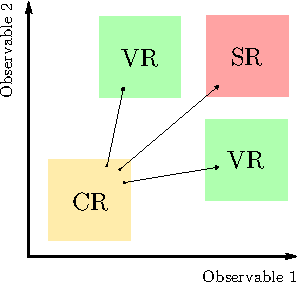
\includegraphics[width=0.40\textwidth]{regions.pdf}
\end{figure}


\begin{itemize}

\item Regiones de Señal (SR): exceso de señal por sobre el fondo predicho por el SM

\item Regiones de Control (CR): normalización de los fondos estimados mediante MC. Cambiando los requisitos de las SRs

\item Regiones de Validación (VR): validación de los fondos calculados. Similares a las SRs pero cambiando/invirtiendo algún criterio

\end{itemize}


\end{frame}



%%%%%%%%%%%%%%%%%%%%%%%%%%%%%%%%%%%%%%%%%%%%%%%%%%%%%%%%%%%%%%%%%%%%%%%%%%%%%%%%%%%%%%%%%%%%%%%%%%%%%%%%%%%%%%



\begin{frame}[fragile]

\frametitle{Resultados típicos observados en búsqueda de SUSY}

\vspace{-0.7cm}

\normalsize

\begin{columns}

\begin{column}{0.45\textwidth}
\centering
\begin{table}
\centering\resizebox{1.\textwidth}{!}{
\begin{tabular}{ l | r | r }

  \hline

  & SR$_{\text{L}}$ & SR$_{\text{H}}$ \\

  \hline

  $N_{\text{fotones}}$  & $> 0$   & $> 0$ \\

  $N_{\text{leptones}}$   & $=0$  & $=0$ \\

  $N_{\text{jets}}$   & $>4$  & $>2$ \\

  $p_{T}^{\text{leading}\: \gamma}$   & $> 145 \text{GeV}$   & $> 400 \text{GeV}$ \\

  $\Delta\phi(\text{jet},\: E_{T}^{\text{miss}})$   & $> 0.4$   & $> 0.4$ \\

  $\Delta\phi(\gamma$,\: $E_{T}^{\text{miss}})$   & $>0.4$  & $>0.4$ \\

  $E_{T}^{\text{miss}} $  & $>200\text{GeV}$   & $>400\text{GeV}$ \\

  $m_{\text{eff}}$  & $> 2000 \text{GeV}$  & $> 2000 \text{GeV}$ \\

  $R_{T}^{4}$   & $< 0.9$   & - \\

  \hline


\end{tabular}}
\end{table}

\begin{figure}

  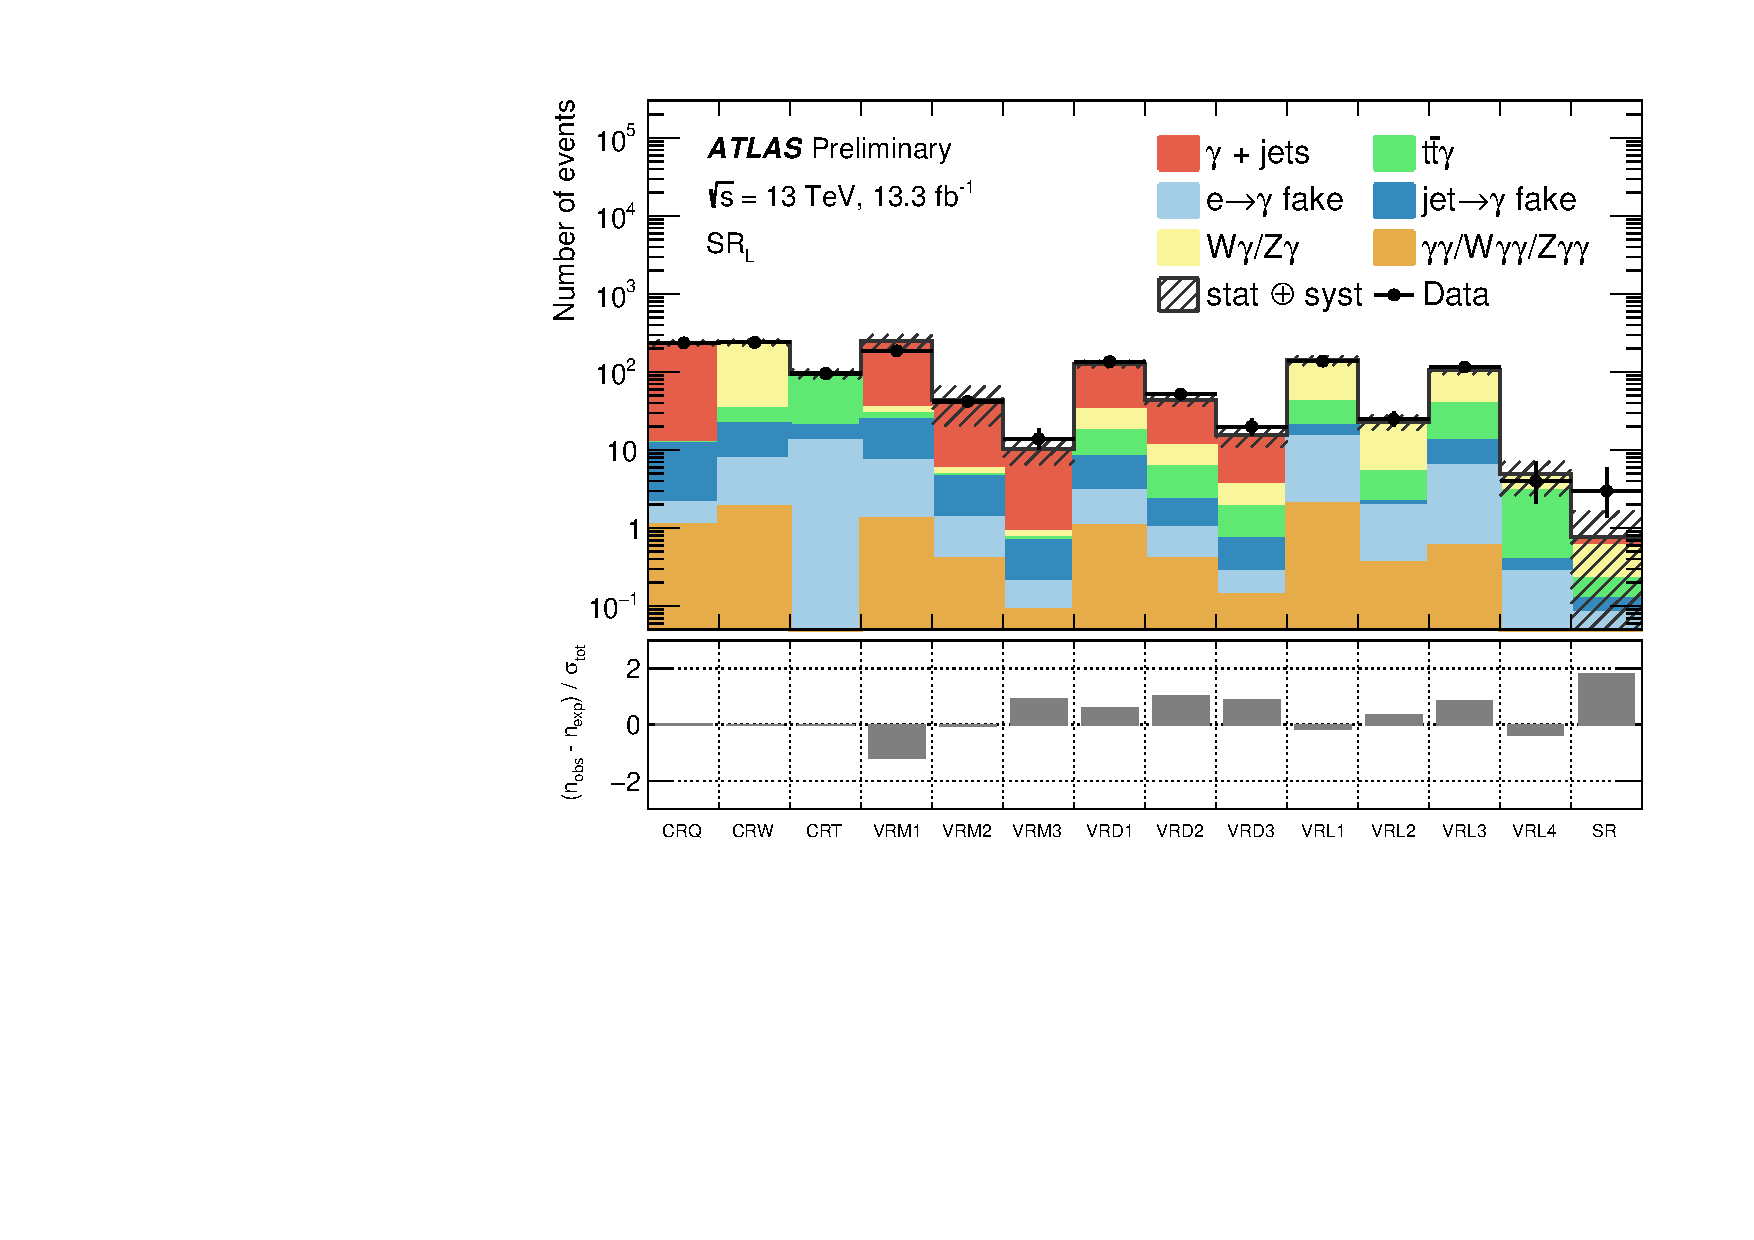
\includegraphics[scale=0.25]{SRL.pdf} 

\end{figure}


\end{column}

\begin{column}{0.45\textwidth}
\centering


\begin{table}
\centering\resizebox{1.1\textwidth}{!}{
\begin{tabular}{ l r r }

  \hline

  SR & SR$_{\text{L}}$ &  SR$_{\text{H}}$ \\

  \hline

  Eventos observados & 3 & 1 \\

  \hline

  Eventos del SM & $0.78 \pm 0.18$ & $1.49 \pm 0.45$\\

  \hline

  $\gamma$ + jets & $0.18 \pm 0.11$ & $0.70 \pm 0.24$\\

  $W\gamma$ & $0.30 \pm 0.07$ & $0.37 \pm 0.09$\\

  $Z\gamma$ & $0.08 \pm 0.08$ & $0.32 \pm 0.32$\\

  $t\bar{t}\gamma$ & $0.10 \pm 0.04$ & $0.03 \pm 0.01$\\

  $e\rightarrow\gamma$ falsos & $0.07 \pm 0.03$ & $0.00 \pm 0.00$\\

  $j\rightarrow\gamma$ falsos & $0.04 \pm 0.01$ & $0.00 \pm 0.00$\\

  $\gamma\gamma / W\gamma\gamma / Z\gamma\gamma$ & $0.01 \pm 0.00$ & $0.07 \pm 0.01$\\

  \hline


\end{tabular}}
\end{table}


\begin{figure}
    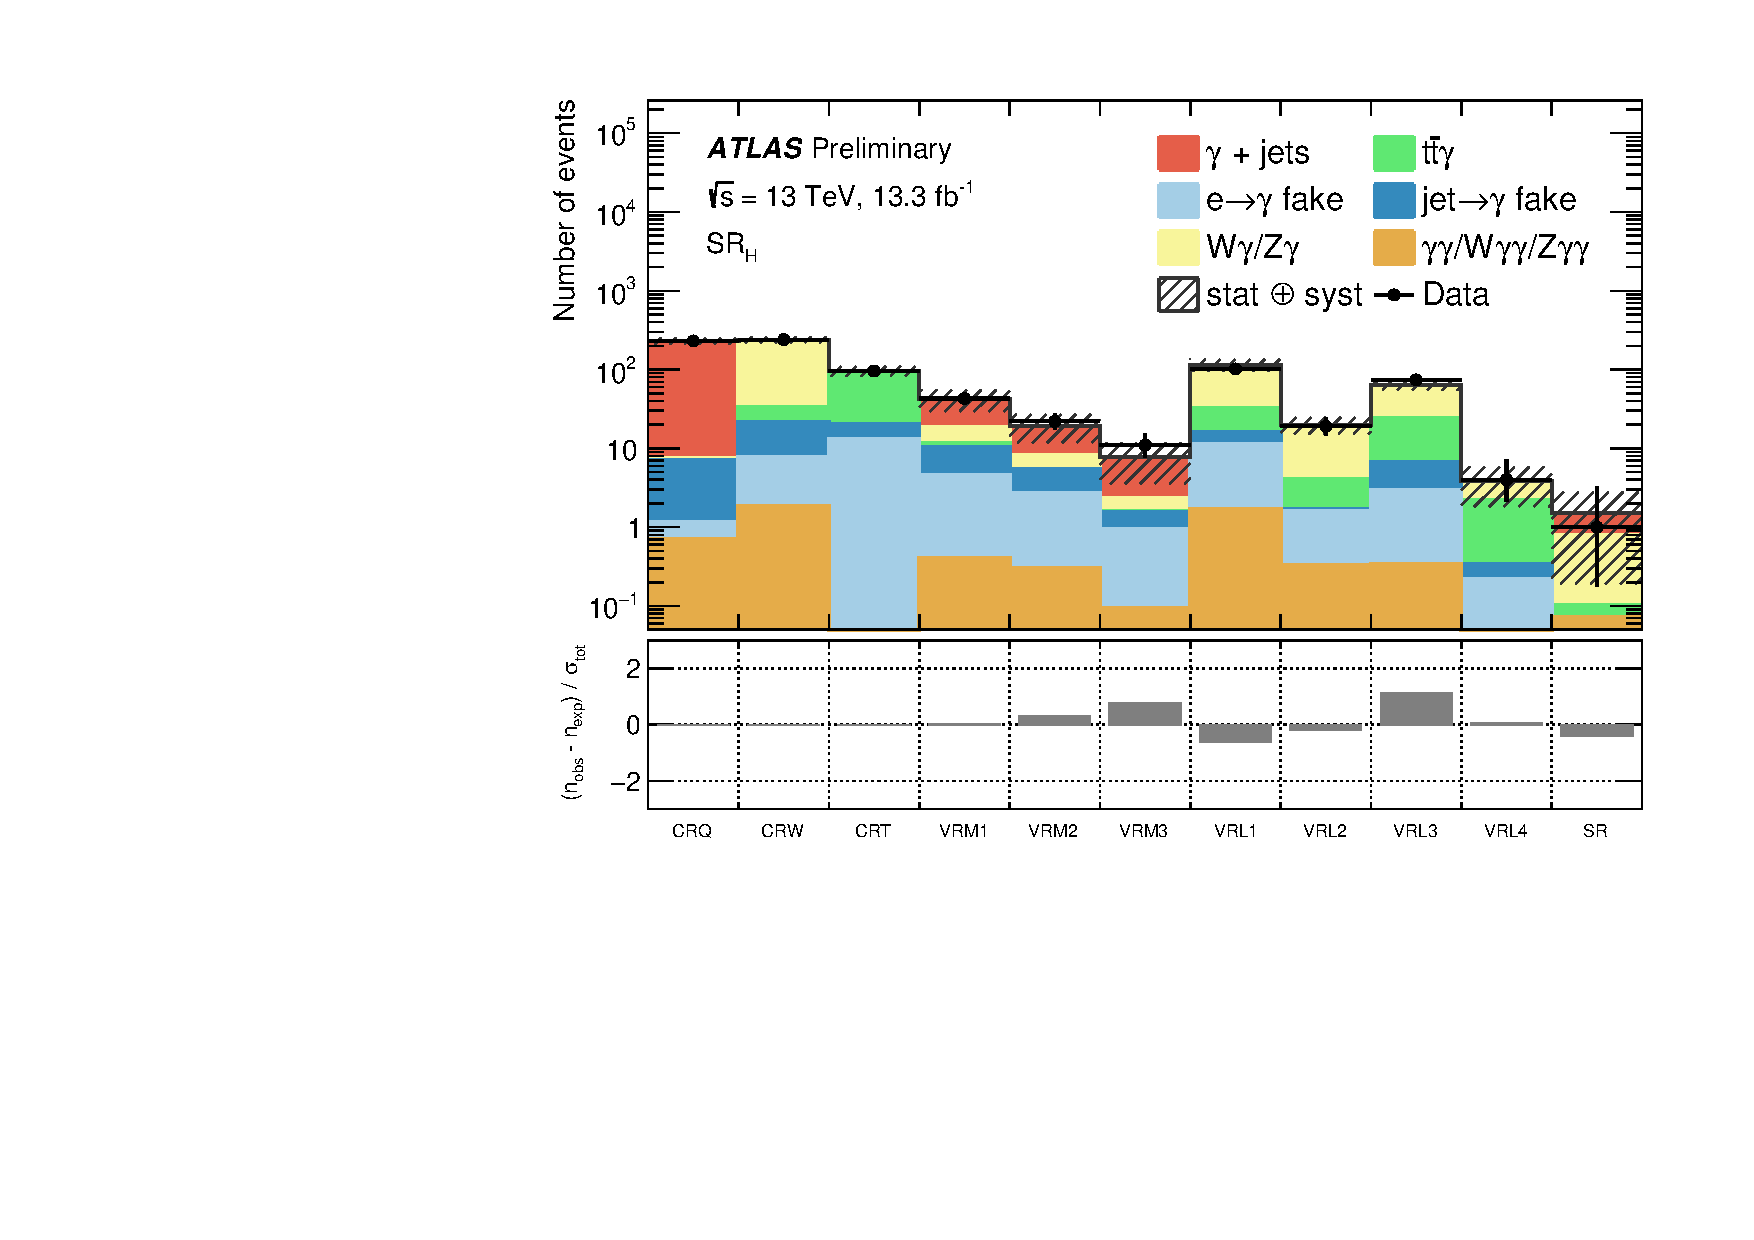
\includegraphics[scale=0.25]{SRH.pdf}
\end{figure}

\end{column}
\end{columns}

\renewcommand{\arraystretch}{1.3}
\tiny Search for Supersymmetry in events with photons, jets and missing transverse energy with the ATLAS detector in 13 TeV pp collisions. ATLAS-CONF-2016-066
\renewcommand{\arraystretch}{1}


\end{frame}



%%%%%%%%%%%%%%%%%%%%%%%%%%%%%%%%%%%%%%%%%%%%%%%%%%%%%%%%%%%%%%%%%%%%%%%%%%%%%%%%%%%%%%%%%%%%%%%%%%%%%%%%%%%%%%


\section{Fondo de electrones mal reconstruidos}
\begin{frame}[fragile]

\frametitle{Fondo de electrones reconstruidos como fotones}

\normalsize
\begin{beamercolorbox}[leftskip=\titlelf]{title}
\usebeamerfont{title} Idea general del método
\end{beamercolorbox}

\normalsize

\begin{itemize}
\item Muestra de eventos de $Z\rightarrow ee$/$Z\rightarrow e\gamma_{\text{falsos}}$

\item Factor de identificación espuria: 
\end{itemize}





\begin{equation*}
F_{e\rightarrow\gamma}[\eta , p_{T}]=\frac{N^{e\gamma}[\eta , p_{T}]}{N^{ee}[\eta , p_{T}]} \label{eq:ff_ratio}
\end{equation*}


\end{frame}



%%%%%%%%%%%%%%%%%%%%%%%%%%%%%%%%%%%%%%%%%%%%%%%%%%%%%%%%%%%%%%%%%%%%%%%%%%%%%%%%%%%%%%%%%%%%%%%%%%%%%%%%%%%%%%



\begin{frame}[fragile]
\frametitle{Selección de objetos}

\normalsize


\begin{block}{Fotones:}
$p_{T} > 25 \text{GeV}$, \textit{tight} y aislados
\end{block}

\begin{block}{Electrones:}
$p_{T} > 25 \text{GeV}$, \textit{tight}/\textit{medium}, \textit{gradient loose}
\end{block}

\vspace{1cm}

\begin{itemize}
\item Fuera de la región del \textit{crack} 

\item $d_{0}$ con una significancia menor a 5, $|\Delta z_{0}\sin\theta|<0.5$ mm

\item Si un electrón y un fotón son reconstruidos con $\sqrt{\Delta\phi^{2}+\Delta\eta^{2}}<0.4$, el fotón es descartado del evento

\item Masa invariante entre $75$ y $105 \text{GeV}$

\item En caso de haber más de un par, se utiliza el que tenga la masa invariante más cercana a la del bosón $Z$

\end{itemize}

\end{frame}




%%%%%%%%%%%%%%%%%%%%%%%%%%%%%%%%%%%%%%%%%%%%%%%%%%%%%%%%%%%%%%%%%%%%%%%%%%%%%%%%%%%%%%%%%%%%%%%%%%%%%%%%%%%%%%


\begin{frame}[fragile]
\frametitle{Descripción analítica del método}

\footnotesize


\begin{itemize}

\item Muestra de \textit{N} pares de electrones y positrones reales

\item $\epsilon_{i}$: eficiencia de reconstruir un electrón, con un valor de $\eta$ y $p_{T}$ correspondientes al bin \textit{i}

\item $f_{ij}$: fracción de pares para los cuales el electrón \textit{leading} (\textit{sub-leading}) está dentro del bin \textit{i} (\textit{j}).

\end{itemize}

Número de eventos en el bin $i$ para los pares $ee$:
\begin{equation*}
N_{i}^{ee} = \sum_{j}\epsilon_{i}\epsilon_{j}f_{ij}N + \sum_{j}\epsilon_{j}\epsilon_{i}f_{ji}N = \epsilon_{i}N\sum_{j}\epsilon_{j}(f_{ij}+f_{ji})
\end{equation*}


\begin{itemize}

\item $p_{i}$ es la proporción de electrones reconstruidos como fotones en el bin \textit{i}

\end{itemize}


Número de eventos en el bin \textit{i} para los pares $e\gamma$:

\begin{equation*}
N_{i}^{e\gamma} = \sum_{j}p_{i}\epsilon_{j}f_{ij}N + \sum_{j}p_{i}\epsilon_{j}f_{ji}N = p_{i}N\sum_{j}\epsilon_{j}(f_{ij}+f_{ji})
\end{equation*}

\begin{equation*}
F_{e\rightarrow\gamma}[\eta , p_{T}]\equiv\frac{N^{e\gamma}}{N^{ee}}=\frac{p_{i}}{\epsilon_{i}}
\end{equation*}


\begin{block}{Número de eventos correspondientes al fondo:}
\begin{equation*}
N_{e\rightarrow\gamma}(\eta , p_{T} , ... ) = F_{e\rightarrow\gamma}(\eta , p_{T})\cdot N_{e}(\eta , p_{T} , ...)
\end{equation*}
\end{block}

\end{frame}





%%%%%%%%%%%%%%%%%%%%%%%%%%%%%%%%%%%%%%%%%%%%%%%%%%%%%%%%%%%%%%%%%%%%%%%%%%%%%%%%%%%%%%%%%%%%%%%%%%%%%%%%%%%%%%


\begin{frame}[fragile]
\frametitle{Distinción entre señal y fondo en eventos $Z\to ee$}

\normalsize



\begin{columns}

\begin{column}{0.5\textwidth}


\begin{block}{Clasificación de eventos:}
Según región de reconstrucción
\begin{itemize}

\item \textit{endcap}-\textit{endcap} ($EE$)

\item \textit{barrel}-\textit{endcap} ($BE$)

\item \textit{barrel}-\textit{barrel} ($BB$)

\end{itemize}

Según tipo
\begin{itemize}

\item $ee$

\item $e\gamma$

\end{itemize}

\begin{block}{Funciones de ajuste:}
\begin{itemize}

\item Señal (S): \textit{double-sided Crystal-ball} (DSCB)

\item Fondo (B): Polinomio de grado 2

\end{itemize}

\end{block}


\end{block}




\end{column}

\begin{column}{0.5\textwidth}

Se define una cantidad:

\begin{equation*}
w=\frac{S}{S+B}
\end{equation*}

\begin{figure}
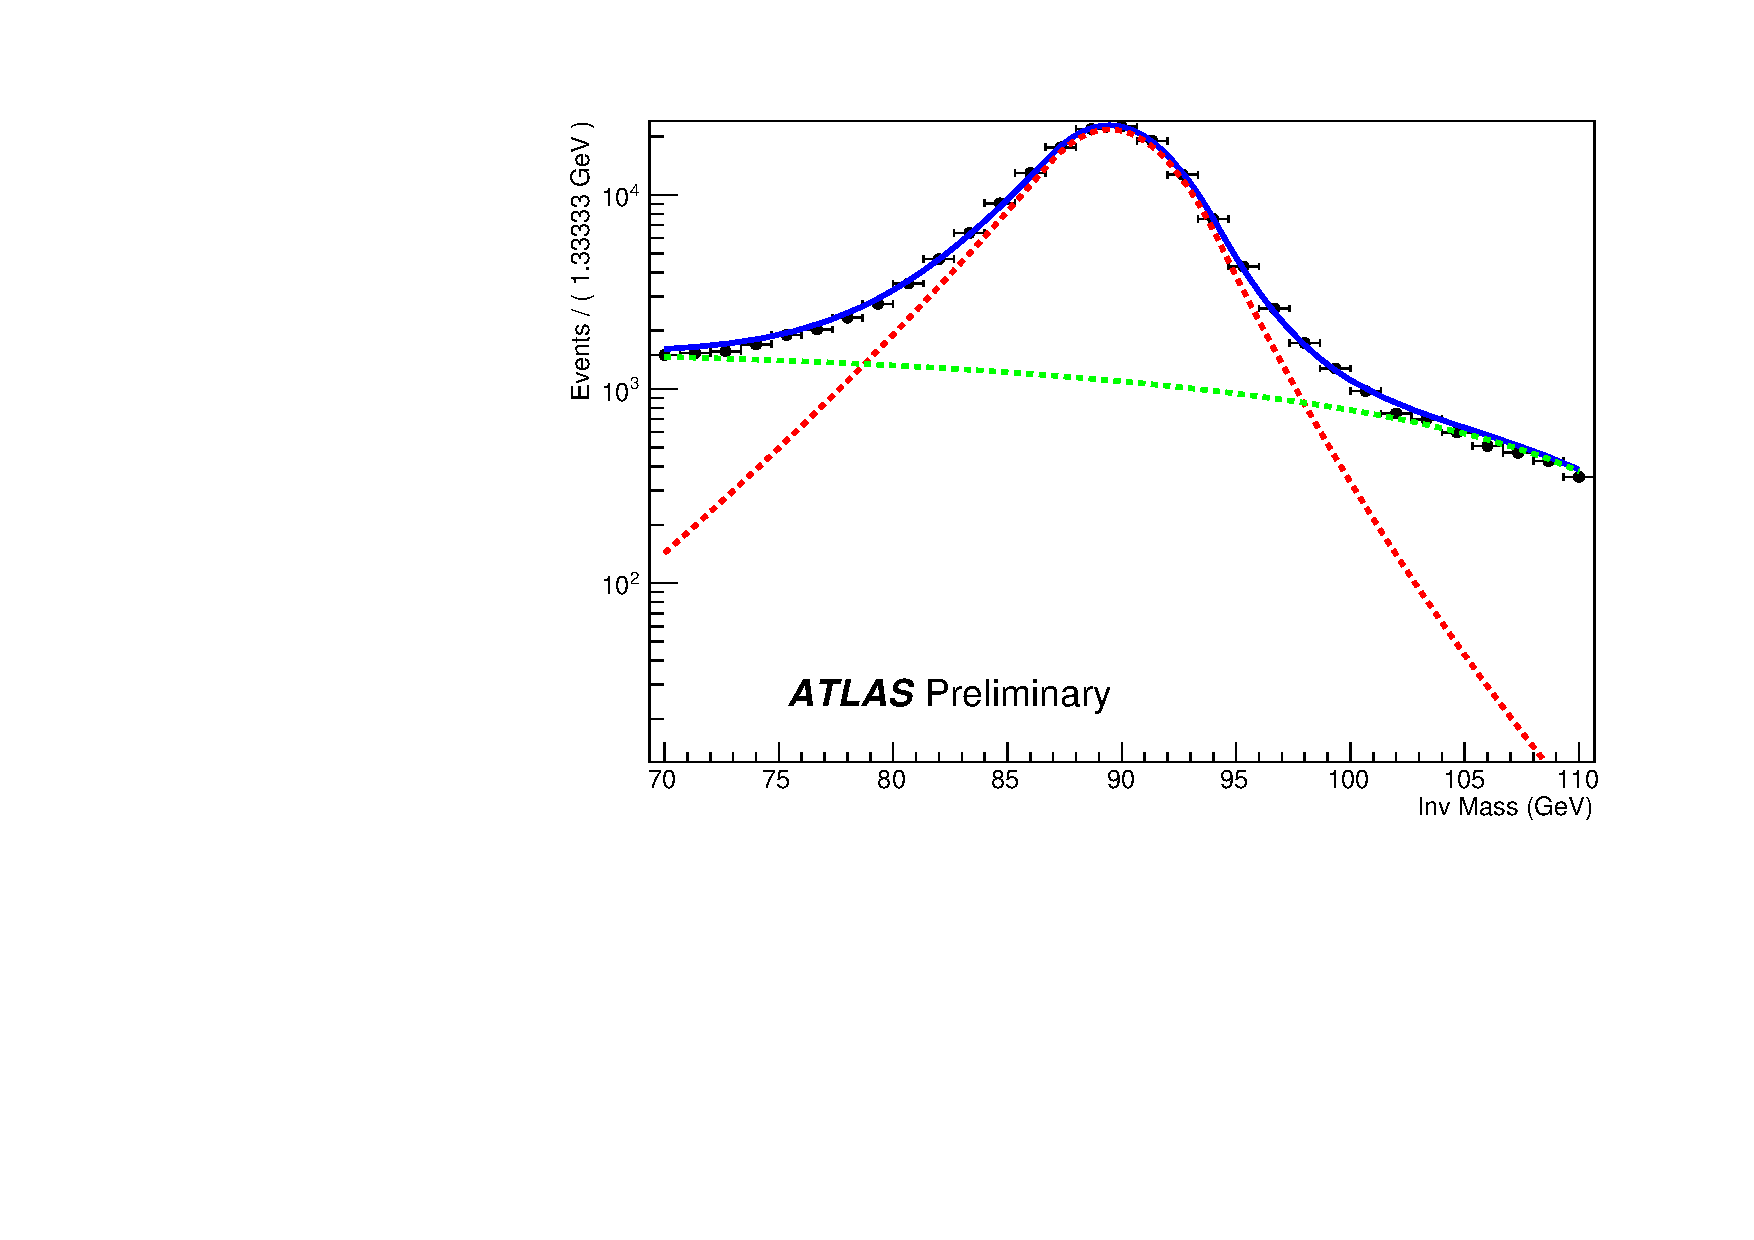
\includegraphics[scale=0.30]{d15_16_egam1_m_lmet_fit_h_m_eg_EE.pdf} 
\end{figure}

{\small {\red DSCB,} {\green Polinomio de grado 2, }{ \blue combinación de ambos}}

\end{column}

\end{columns}


\end{frame}


%%%%%%%%%%%%%%%%%%%%%%%%%%%%%%%%%%%%%%%%%%%%%%%%%%%%%%%%%%%%%%%%%%%%%%%%%%%%%%%%%%%%%%%%%%%%%%%%%%%%%%%%%%%%%%


\begin{frame}[fragile]

\normalsize

\begin{columns}

\begin{column}{0.5\textwidth}

\vspace{-1cm}

\begin{table}
\centering\resizebox{1.3\textwidth}{!}{
\begin{tabular}{ c c c | c c }

  \hline
  \hline

  \multirow{2}{*}{Región} & \multicolumn{2}{c |}{\textit{medium e}} & \multicolumn{2}{c}{\textit{tight e}} \\

  \cline{2-5}

   & $ee$ & $e\gamma$ & $ee$ & $e\gamma$ \\

  \hline

  EE & 0.915(2) & 0.810(7)  & 0.928(2) & 0.817(7) \\

  BE & 0.937(1) & 0.800(4)  & 0.934(1) & 0.812(5) \\

  BB & 0.9175(7) & 0.722(4)  & 0.9155(8) & 0.734(4) \\

  \hline
  \hline
\end{tabular}}
\end{table}

\vspace{2cm}

Para pares cuya masa invariante este dentro del rango $[75-105]\text{GeV}$:

\begin{equation*}
F_{e\rightarrow\gamma}[\eta , p_{T}]=\frac{N^{e\gamma}_{\text{pesado}}}{N^{ee}_{\text{pesado}}}
\end{equation*}


\end{column}

\begin{column}{0.5\textwidth}

\begin{figure}
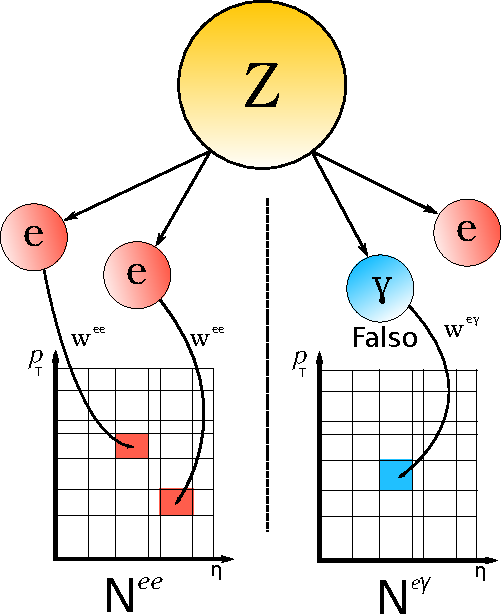
\includegraphics[width=1\textwidth]{grid.pdf}
\end{figure}


\end{column}

\end{columns}





\end{frame}

%%%%%%%%%%%%%%%%%%%%%%%%%%%%%%%%%%%%%%%%%%%%%%%%%%%%%%%%%%%%%%%%%%%%%%%%%%%%%%%%%%%%%%%%%%%%%%%%%%%%%%%%%%%%%%


\begin{frame}[fragile]
% \frametitle{Incertezas sistemáticas}

\normalsize



\begin{beamercolorbox}[leftskip=\titlelf]{title}
\usebeamerfont{title}\normalsize Incertezas sistemáticas
\end{beamercolorbox}

\begin{itemize}

\item Variando los rangos de masa de aceptación de pares: de $[75-105]\text{GeV}$ a los rangos de $[70-110]\text{GeV}$ y a $[80-100]\text{GeV}$

\item Sin la sustracción de fondo fijando el peso $w=1$

\end{itemize}

\vspace{1.5cm}

El sistemático proveniente de $w=1$ es el que predomina siendo de un $20\%$

\end{frame}



%%%%%%%%%%%%%%%%%%%%%%%%%%%%%%%%%%%%%%%%%%%%%%%%%%%%%%%%%%%%%%%%%%%%%%%%%%%%%%%%%%%%%%%%%%%%%%%%%%%%%%%%%%%%%%


\begin{frame}[fragile]
\frametitle{Resultados de factores}

\normalsize

\begin{table} 
\centering\resizebox{1.\textwidth}{!}{
\begin{tabular}{  l l | c c c c c | c c c c c}

  \hline
  \hline

  & & \multicolumn{5}{c |}{\textit{medium}} & \multicolumn{5}{c }{\textit{tight}} \\

  \cline{3-12}

  \multirow{1}{*}{$|\eta|$} & \multirow{1}{*}{$p_{T}$[GeV]} & \multirow{2}{*}{Fake factor} & \multirow{2}{*}{Estadístico} & \multicolumn{3}{c |}{Sistemáticos}  & \multirow{2}{*}{Fake factor} & \multirow{2}{*}{Estadístico} & \multicolumn{3}{c }{Sistemáticos}\\

  \cline{5-7}\cline{10-12}

      & & &   & $w=1$ & Rango & Total &   &  & $w=1$ & Rango & Total \\


  \hline
  \hline

  0 - 0.6   & 75 - 90   & 0.0149 & 0.0003 & 0.004 &  0.0004 &  0.004  & 0.0155 & 0.0004 & 0.004 &  0.001  &  0.004  \\

  0 - 0.6   & 90 - 145  & 0.0136 & 0.0004 & 0.004 &  0.0004 &  0.004  & 0.0141 & 0.0004 & 0.004 &  0.002  &  0.004  \\

  0 - 0.6   & 145 - 300 & 0.0113 & 0.0008 & 0.003 &  0.0003 &  0.003  & 0.0116 & 0.0008 & 0.002 &  0.001  &  0.003  \\

  \hline

  0.6 - 1.37  & 75 - 90   & 0.0164 & 0.0003 & 0.004 &  0.0004 &  0.004  & 0.0173 & 0.0004 & 0.004 &  0.002  &  0.004  \\

  0.6 - 1.37  & 90 - 145  & 0.0157 & 0.0004 & 0.004 &  0.0003 &  0.004  & 0.0161 & 0.0004 & 0.004 &  0.002  &  0.004  \\

  0.6 - 1.37  & 145 - 300 & 0.0116 & 0.0007 & 0.003 &  0.0003 &  0.003  & 0.0121 & 0.0008 & 0.003 &  0.002  &  0.003  \\

  \hline

  1.52 - 1.82 & 75 - 90   & 0.034  & 0.001 & 0.005  &  0.0005 &  0.005  & 0.036  & 0.001 & 0.005  &  0.002  &  0.005 \\

  1.52 - 1.82 & 90 - 145  & 0.030  & 0.001 & 0.005  &  0.001  &  0.005  & 0.033  & 0.001 & 0.004  &  0.003  &  0.005  \\

  1.52 - 1.82 & 145 - 300 & 0.023  & 0.002 & 0.003  &  0.0005 &  0.003  & 0.022  & 0.002 & 0.003  &  0.001  &  0.003  \\

  \hline

  1.82 - 2.37 & 75 - 90   & 0.044   & 0.001 & 0.006 &  0.002  &  0.006  & 0.046   & 0.001 & 0.007 &  0.002  &  0.007  \\

  1.82 - 2.37 & 90 - 145  & 0.038   & 0.001 & 0.005 &  0.001  &  0.005  & 0.039   & 0.001 & 0.006 &  0.003  &  0.007  \\

  1.82 - 2.37 & 145 - 300 & 0.039   & 0.003 & 0.006 &  0.001  &  0.006  & 0.041   & 0.003 & 0.006 &  0.002  &  0.006  \\

  \hline
  \hline

\end{tabular}}
\end{table}

Electrones \textit{tight}: mayor pureza

Electrones \textit{medium}: mayor estadística

\hrulefill

Sistemáticos similares $\longrightarrow$ se optó por utilizar electrones \textit{medium}

\end{frame}



%%%%%%%%%%%%%%%%%%%%%%%%%%%%%%%%%%%%%%%%%%%%%%%%%%%%%%%%%%%%%%%%%%%%%%%%%%%%%%%%%%%%%%%%%%%%%%%%%%%%%%%%%%%%%%


\begin{frame}[fragile]
\frametitle{Validación de los resultados obtenidos}

\normalsize
\vspace{-0.5cm}
\begin{columns}

\begin{column}{0.45\textwidth}
\begin{table}
\centering\resizebox{0.9\textwidth}{!}{
  \begin{tabular}{l|r}
  \hline
  \hline
  & VRE \\
  \hline
  $N_{\mathrm{fotones}}$                  &       $\ge1$  \\
  $p_{T}^{\text{leading}\: \gamma} >$         &    $145\text{GeV}$  \\
  $N_{\mathrm{leptones}}$                  &           -   \\
  $N_{\mathrm{jets}}$                     &       $\ge1$  \\
  $N_{b-\mathrm{jets}}$                   &       $\ge1$  \\
  $\Delta\phi(\text{jet}, E_{T}^{\text{miss}})$          &       $>0.4$  \\
  $\Delta\phi(\gamma, E_{T}^{\text{miss}})$                &       $<0.4$  \\
  ${E_{T}^{\text{miss}}}$                                &   $>200\text{GeV}$  \\
  $m_{\text{eff}}$                               &  $[500, 2000]\text{GeV}$  \\
  \hline
  \hline
\end{tabular}}

\end{table}

\begin{table}
\centering\resizebox{1\textwidth}{!}{
\begin{tabular}{lr}
\hline
 & $e\to\gamma$ falsos VR \\
\hline
Eventos observados & 94 \\
\hline
Eventos esperados por el SM & $92.18 \pm 12.58$ \\
\hline
$\gamma$ + jets & $1.46 \pm 0.16$ \\
$W\gamma$ & $13.73 \pm 1.26$ \\
$Z\gamma$ & $0.87 \pm 0.05$ \\
$t\bar{t}\gamma$ & $4.91 \pm 0.70$ \\
$e\rightarrow\gamma$ falsos & $58.43 \pm 12.49$ \\
$\text{jets}\rightarrow\gamma$ falsos & $12.73 \pm 2.14$ \\
$\gamma\gamma / W\gamma\gamma / Z\gamma\gamma$ & $0.05 \pm 0.00$ \\
\hline
\end{tabular}}
\end{table}
\end{column}

\begin{column}{0.45\textwidth}
\begin{figure}
\centering
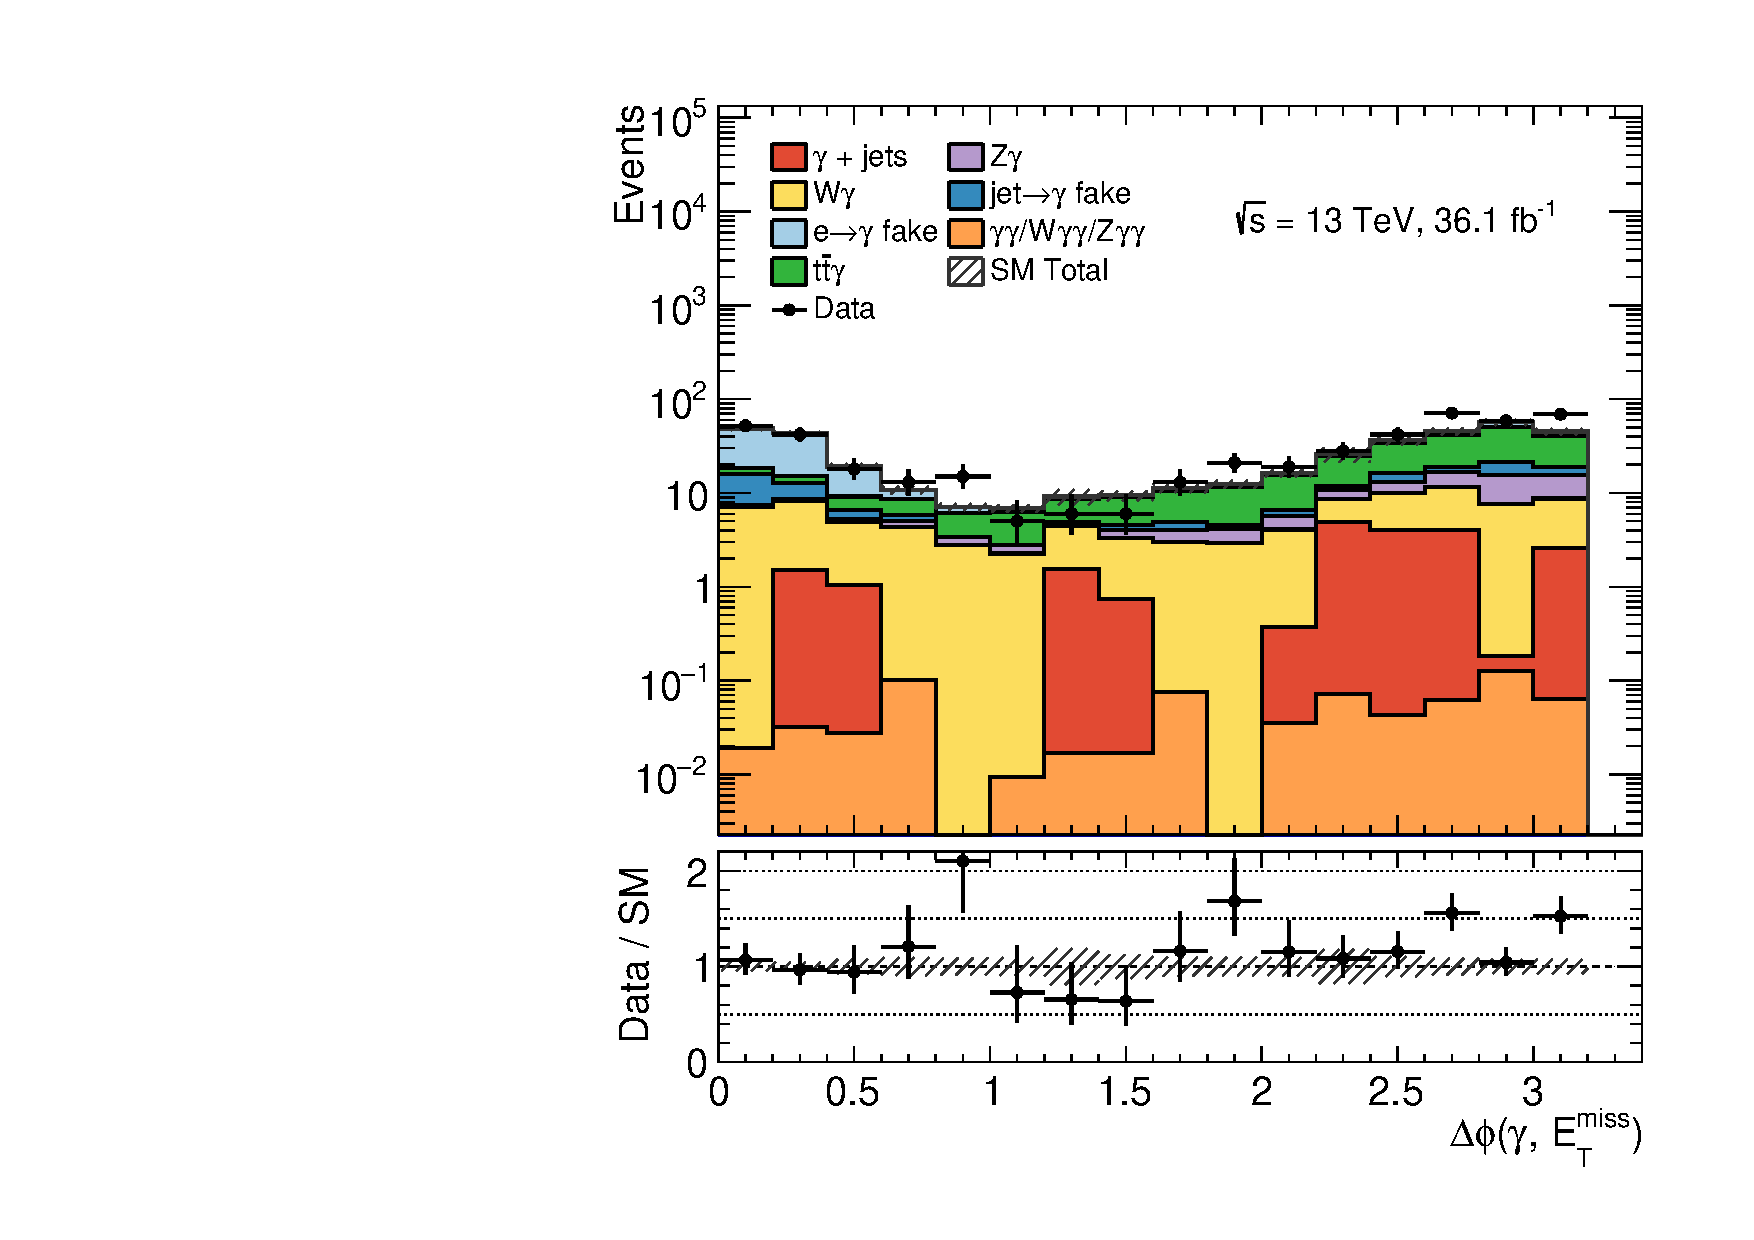
\includegraphics[width=0.85\textwidth]{can_VRE_dphi_gammet_afterFit.pdf}
\end{figure}
\vspace{-0.8cm}
\begin{figure}
\centering
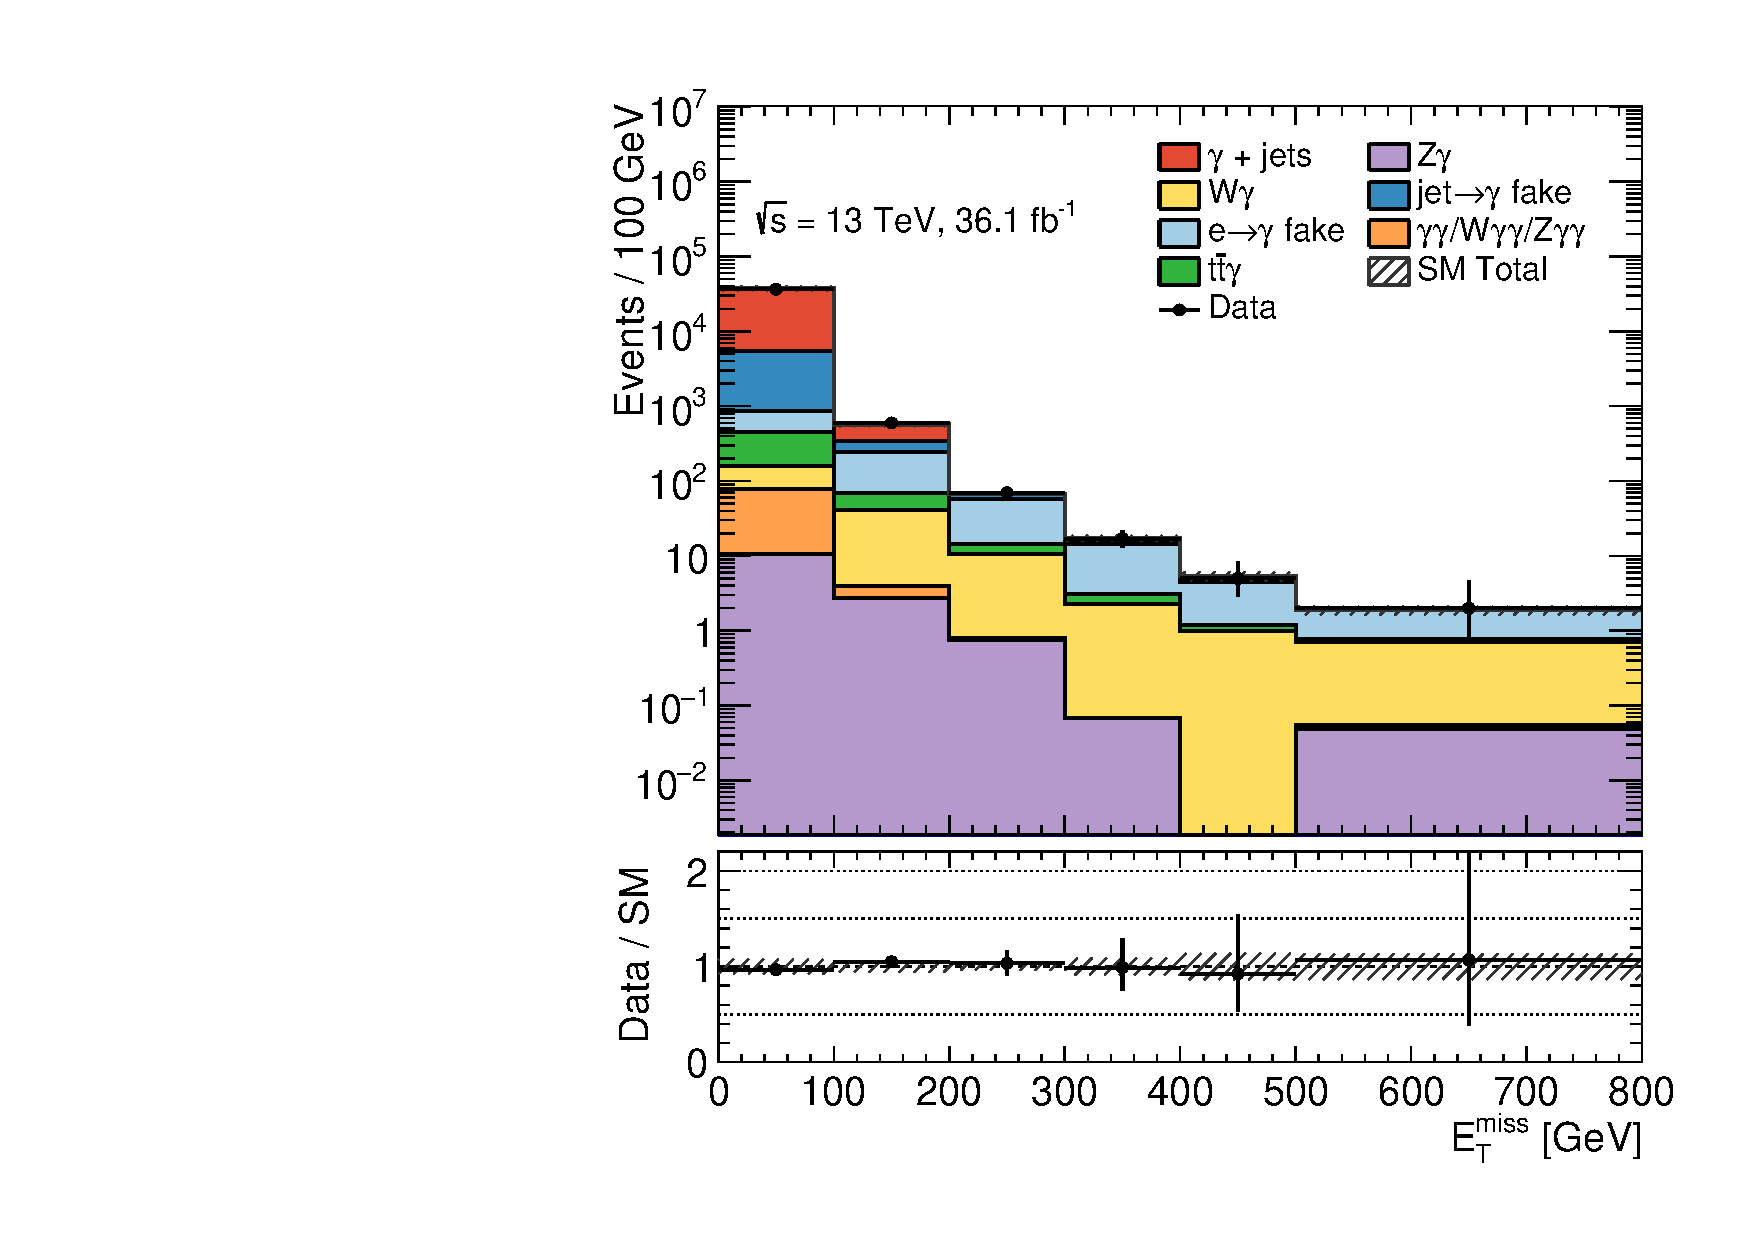
\includegraphics[width=0.85\textwidth]{can_VRE_met_et_afterFit.pdf}
\end{figure}
\end{column}

\end{columns}



\end{frame}



%%%%%%%%%%%%%%%%%%%%%%%%%%%%%%%%%%%%%%%%%%%%%%%%%%%%%%%%%%%%%%%%%%%%%%%%%%%%%%%%%%%%%%%%%%%%%%%%%%%%%%%%%%%%%%

\section{Conclusiones}
\begin{frame}[fragile]
\frametitle{Conclusiones}

\normalsize

\begin{itemize}

\item Se implementó un método para poder estimar procesos donde un electrón del estado final es reconstruido como un fotón, con datos colectados por el detector ATLAS durante el Run 2 del LCH en los años 2015 y 2016.

\item Verificados en una nueva región de validación

\item Compatibles con predicciones en base a datos del 2015 y técnicas anteriores

\item Estudios de criterios de identificación de los electrones tanto \textit{medium} como \textit{tight}, se optó por utilizar \textit{medium}

\end{itemize}


\vspace{1cm}


\begin{beamercolorbox}[leftskip=\titlelf]{title}
\centering\usebeamerfont{title}\large ¡Los resultados están siendo implementados actualmente por la colaboración ATLAS!
\end{beamercolorbox}


\end{frame}



%%%%%%%%%%%%%%%%%%%%%%%%%%%%%%%%%%%%%%%%%%%%%%%%%%%%%%%%%%%%%%%%%%%%%%%%%%%%%%%%%%%%%%%%%%%%%%%%%%%%%%%%%%%%%%




\end{document}
